	\begin{frame}
	\frametitle{День 10. 27 августа}
	\framesubtitle{\textbf{пер. Перемётный (1А, 3255)}~--- д.р. Танышхан} % Optional subtitle
	\begin{columns}[c] % The "c" option specifies centered vertical alignment while the "t" option is used for top vertical alignment
		\begin{column}{0.55\textwidth} % Left column width
			\begin{itemize}
				\item Куда укажет флюгер
				\item Клад для руковода
				\item Косяк руковода
				\item Первая кровь
				\item Тот самый спуск с Перемётного
				\item Последствия ошибки руковода
				\item Прошли \textbf{7.1} км
				\item ЧХВ: 6:50
				\item Набор/сброс: \textcolor{darkred}{\textbf{+575}}/\textcolor{darkblue}{\textbf{-935}}~м
			\end{itemize}
			
		\end{column}
		\begin{column}{0.45\textwidth} % Right column width
			\centering
			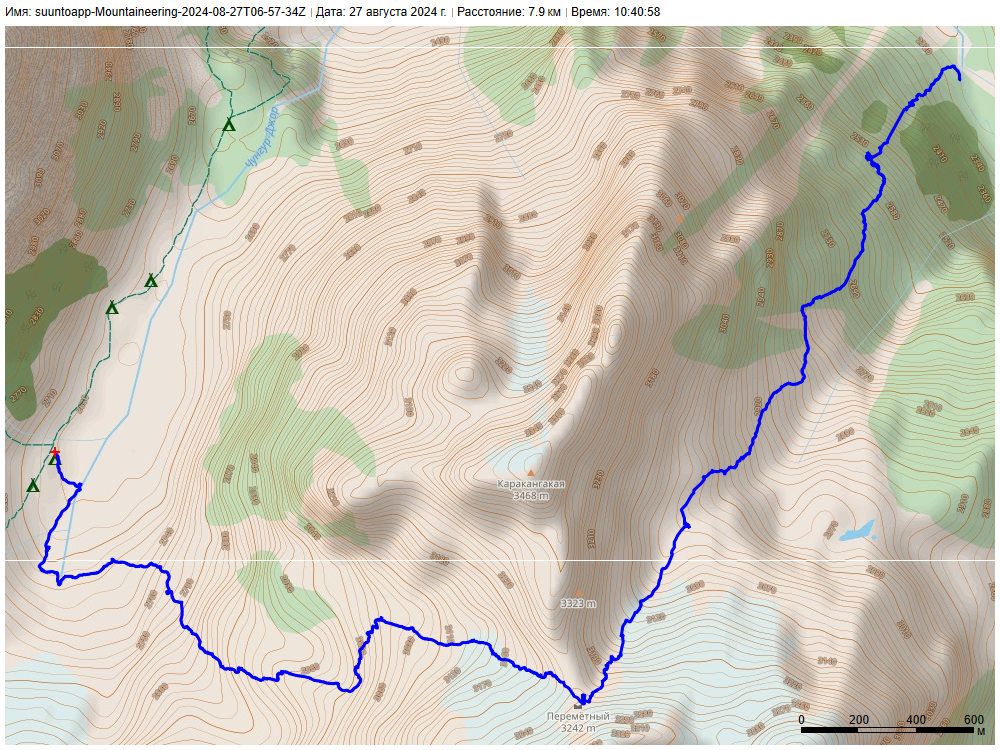
\includegraphics[width=\linewidth]{../pics/mini_maps/27}
		\end{column}
	\end{columns}
\end{frame}

\begin{frame}
	\frametitle{Стойбище}
	\framesubtitle{День 10, 27 августа}
	\centering
	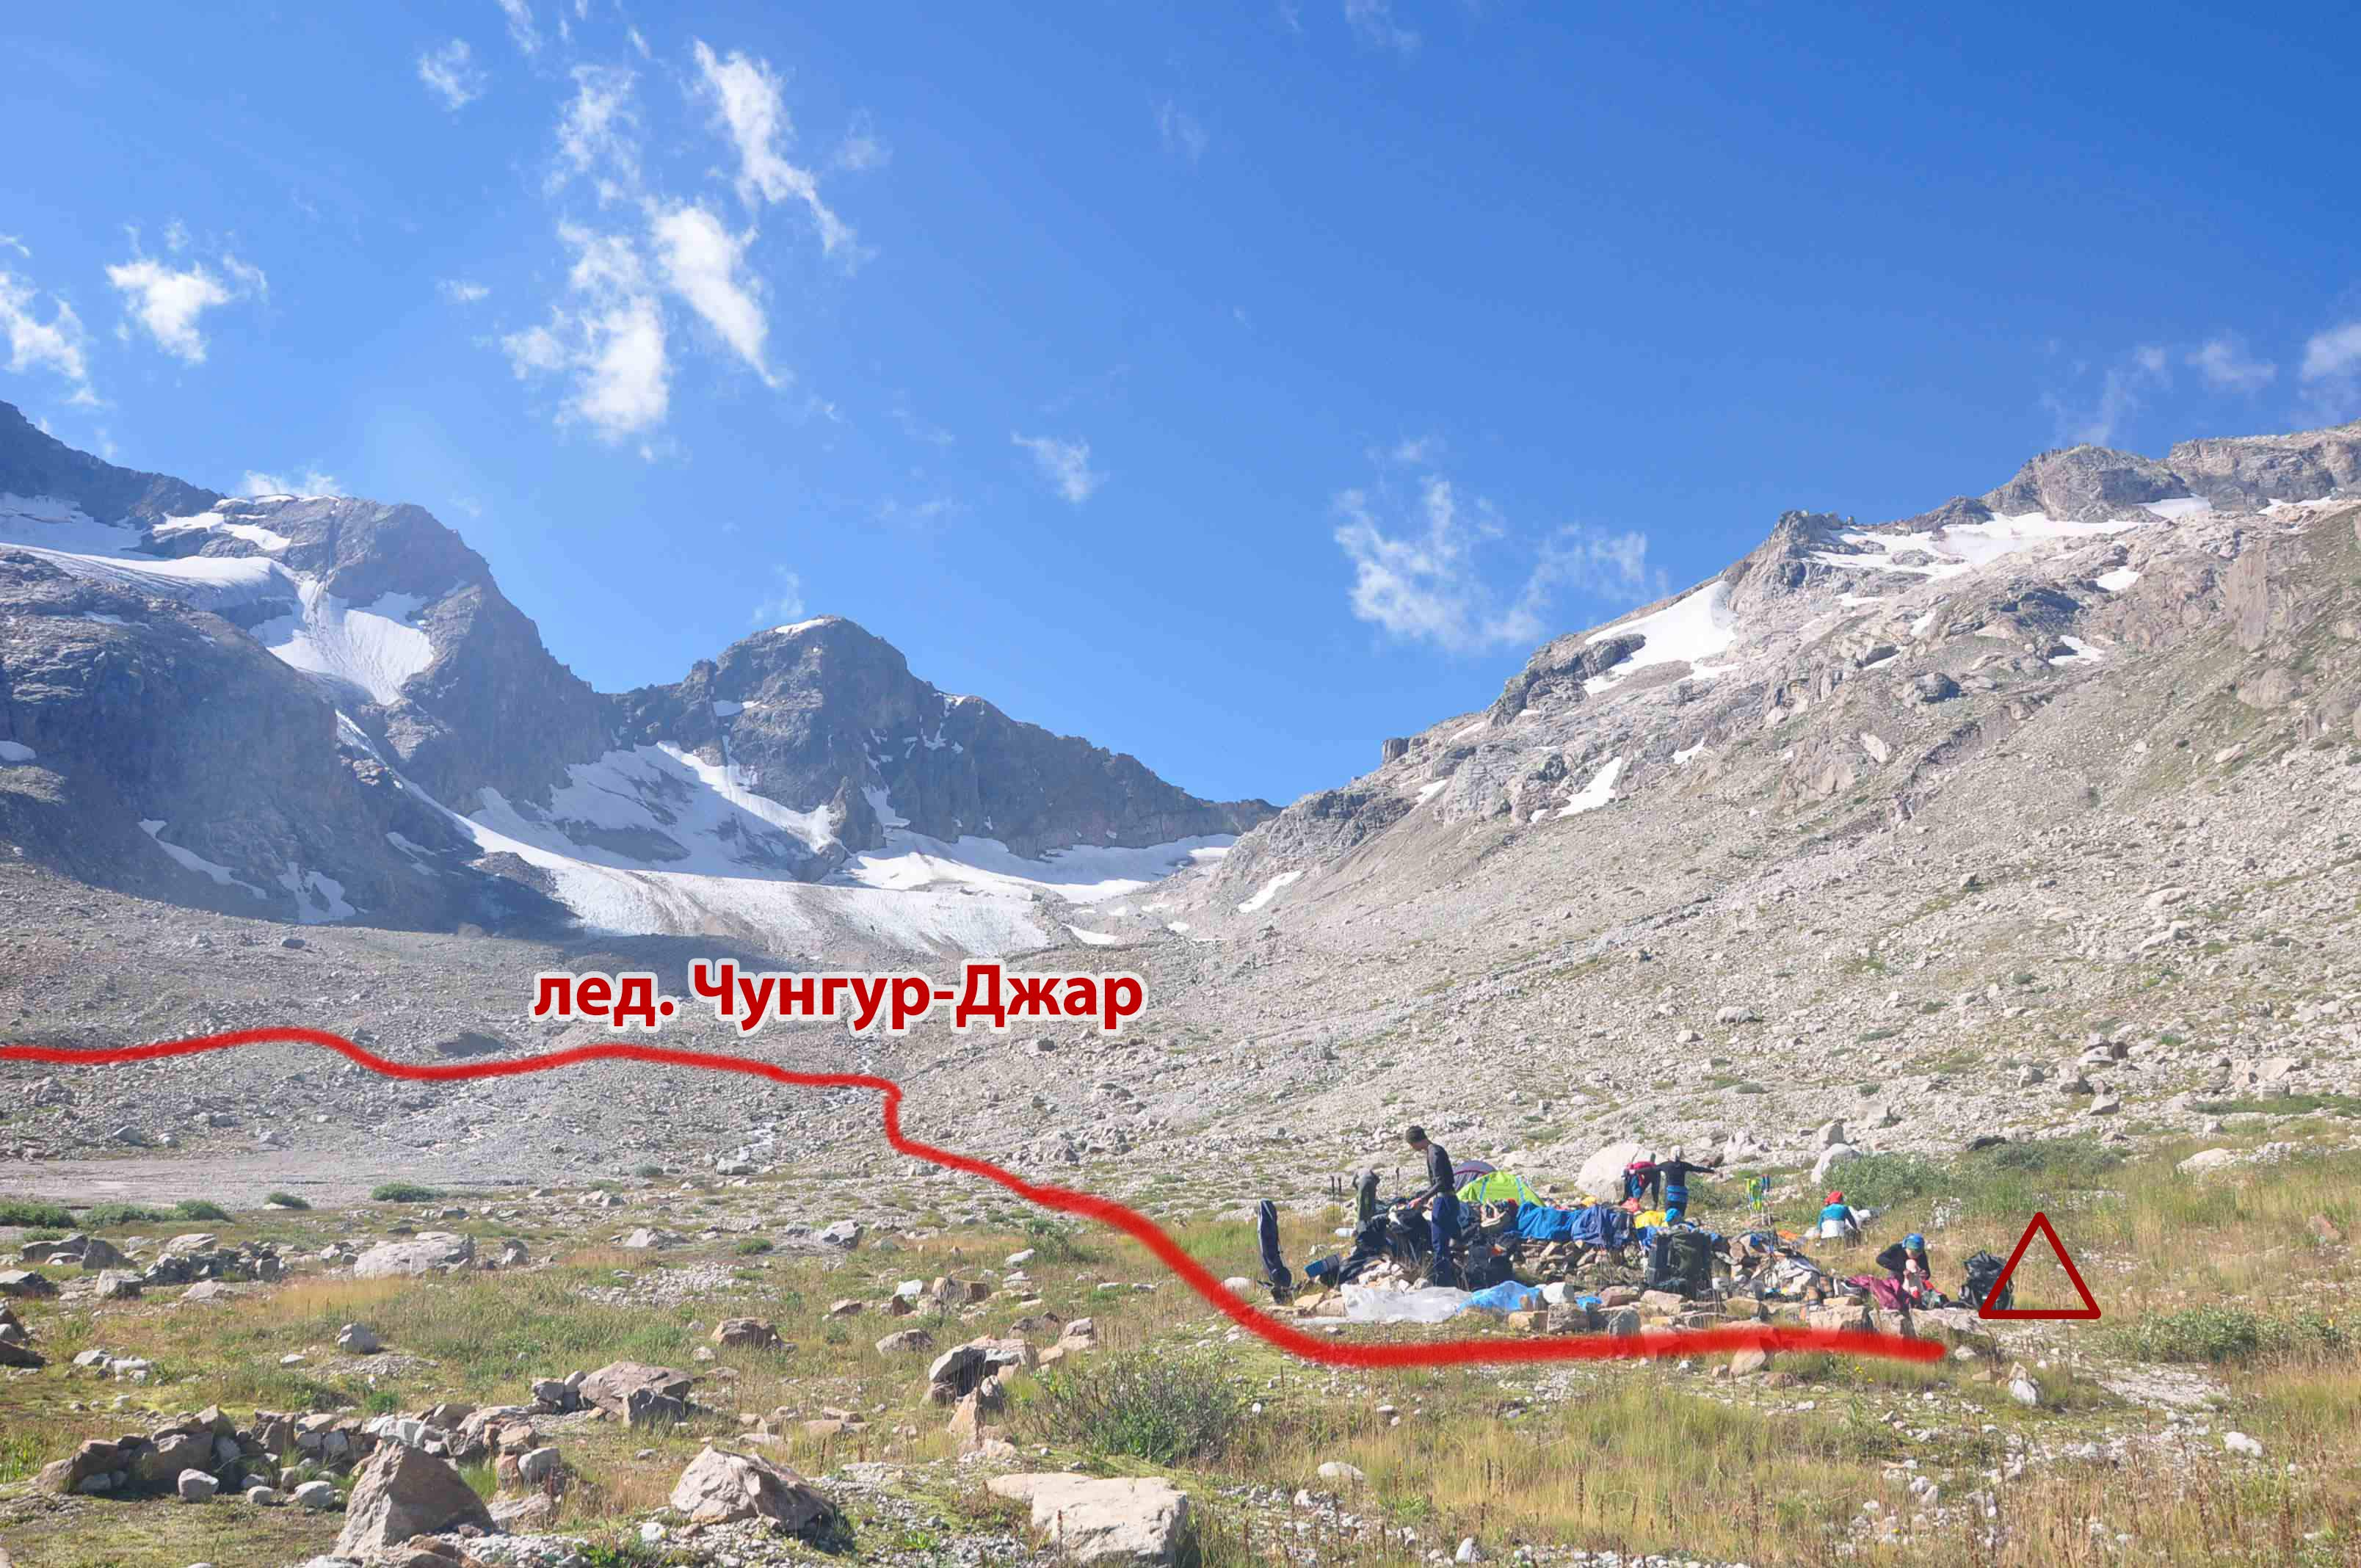
\includegraphics[width=\textwidth]{../pics/DSC_0252}			
\end{frame}

\begin{frame}
	\frametitle{р. Чунгур-Джар. Нам предстоит перебраться через множество ручейков}
	\framesubtitle{День 10, 27 августа}
	\centering
	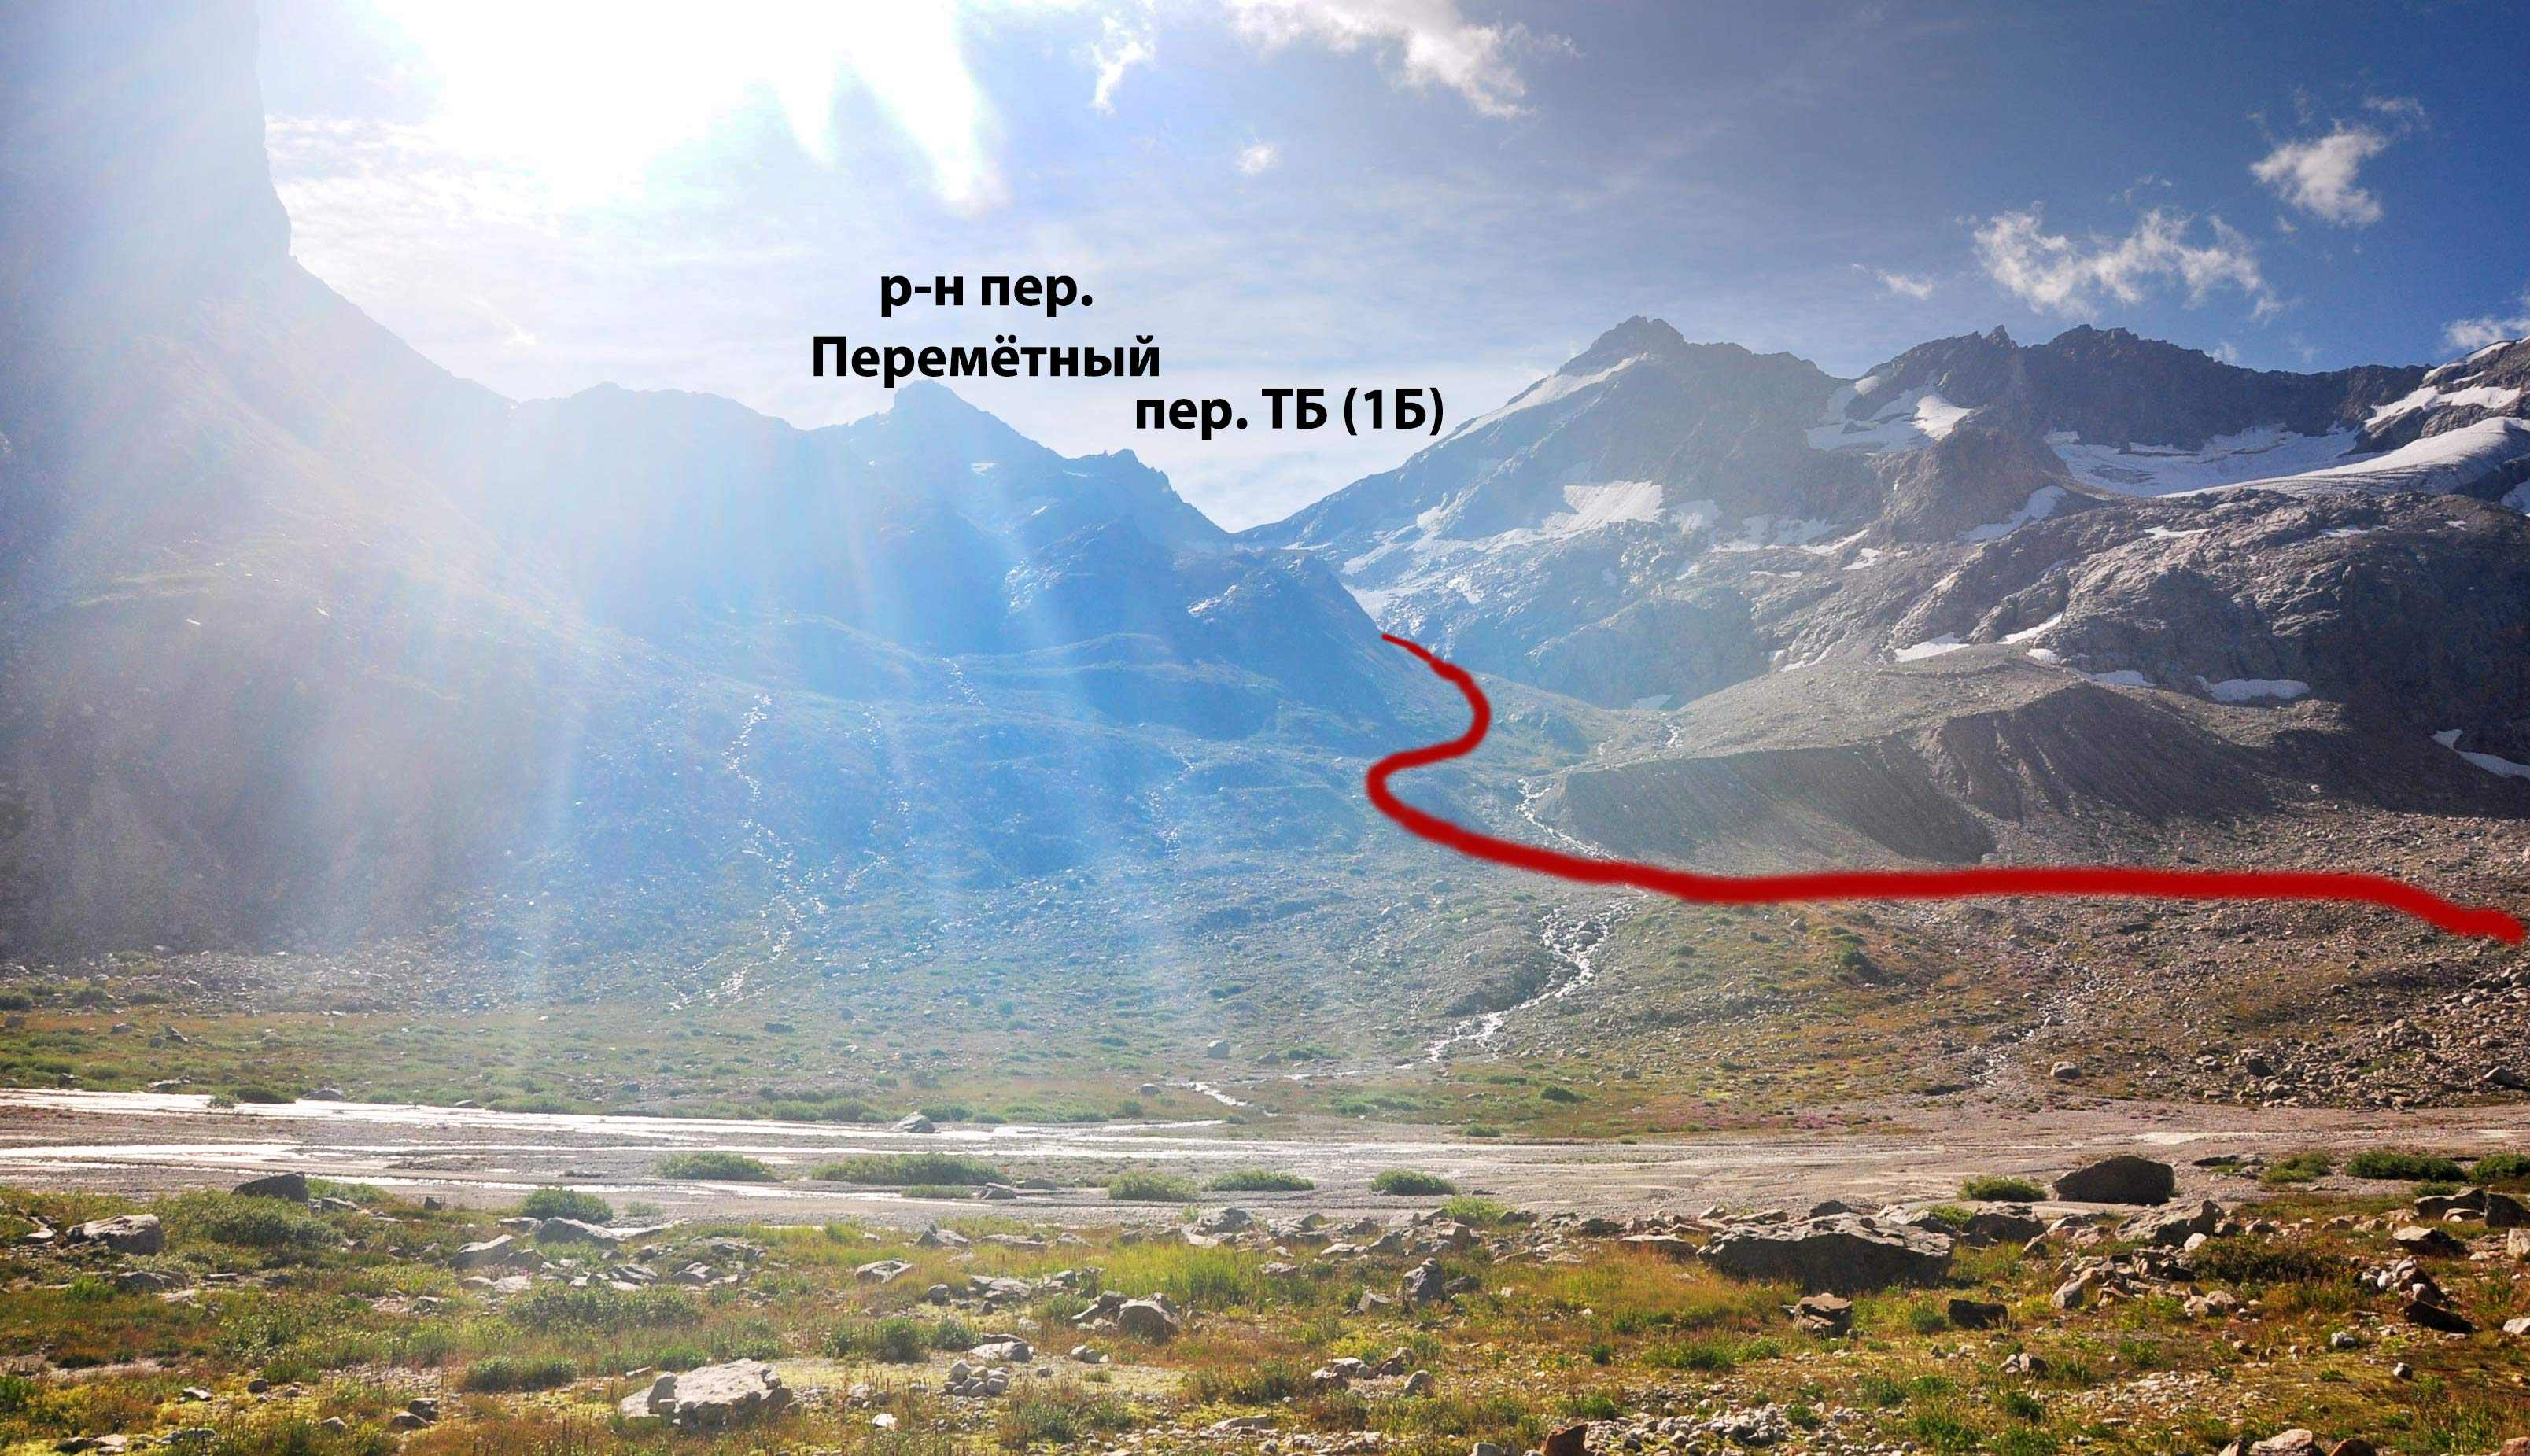
\includegraphics[width=\textwidth]{../pics/DSC_0254}			
\end{frame}

\begin{frame}
	\frametitle{Начало подъёма к пер. Перемётный из д.р. Чунгур-Джар}
	\framesubtitle{День 10, 27 августа}
	\centering
	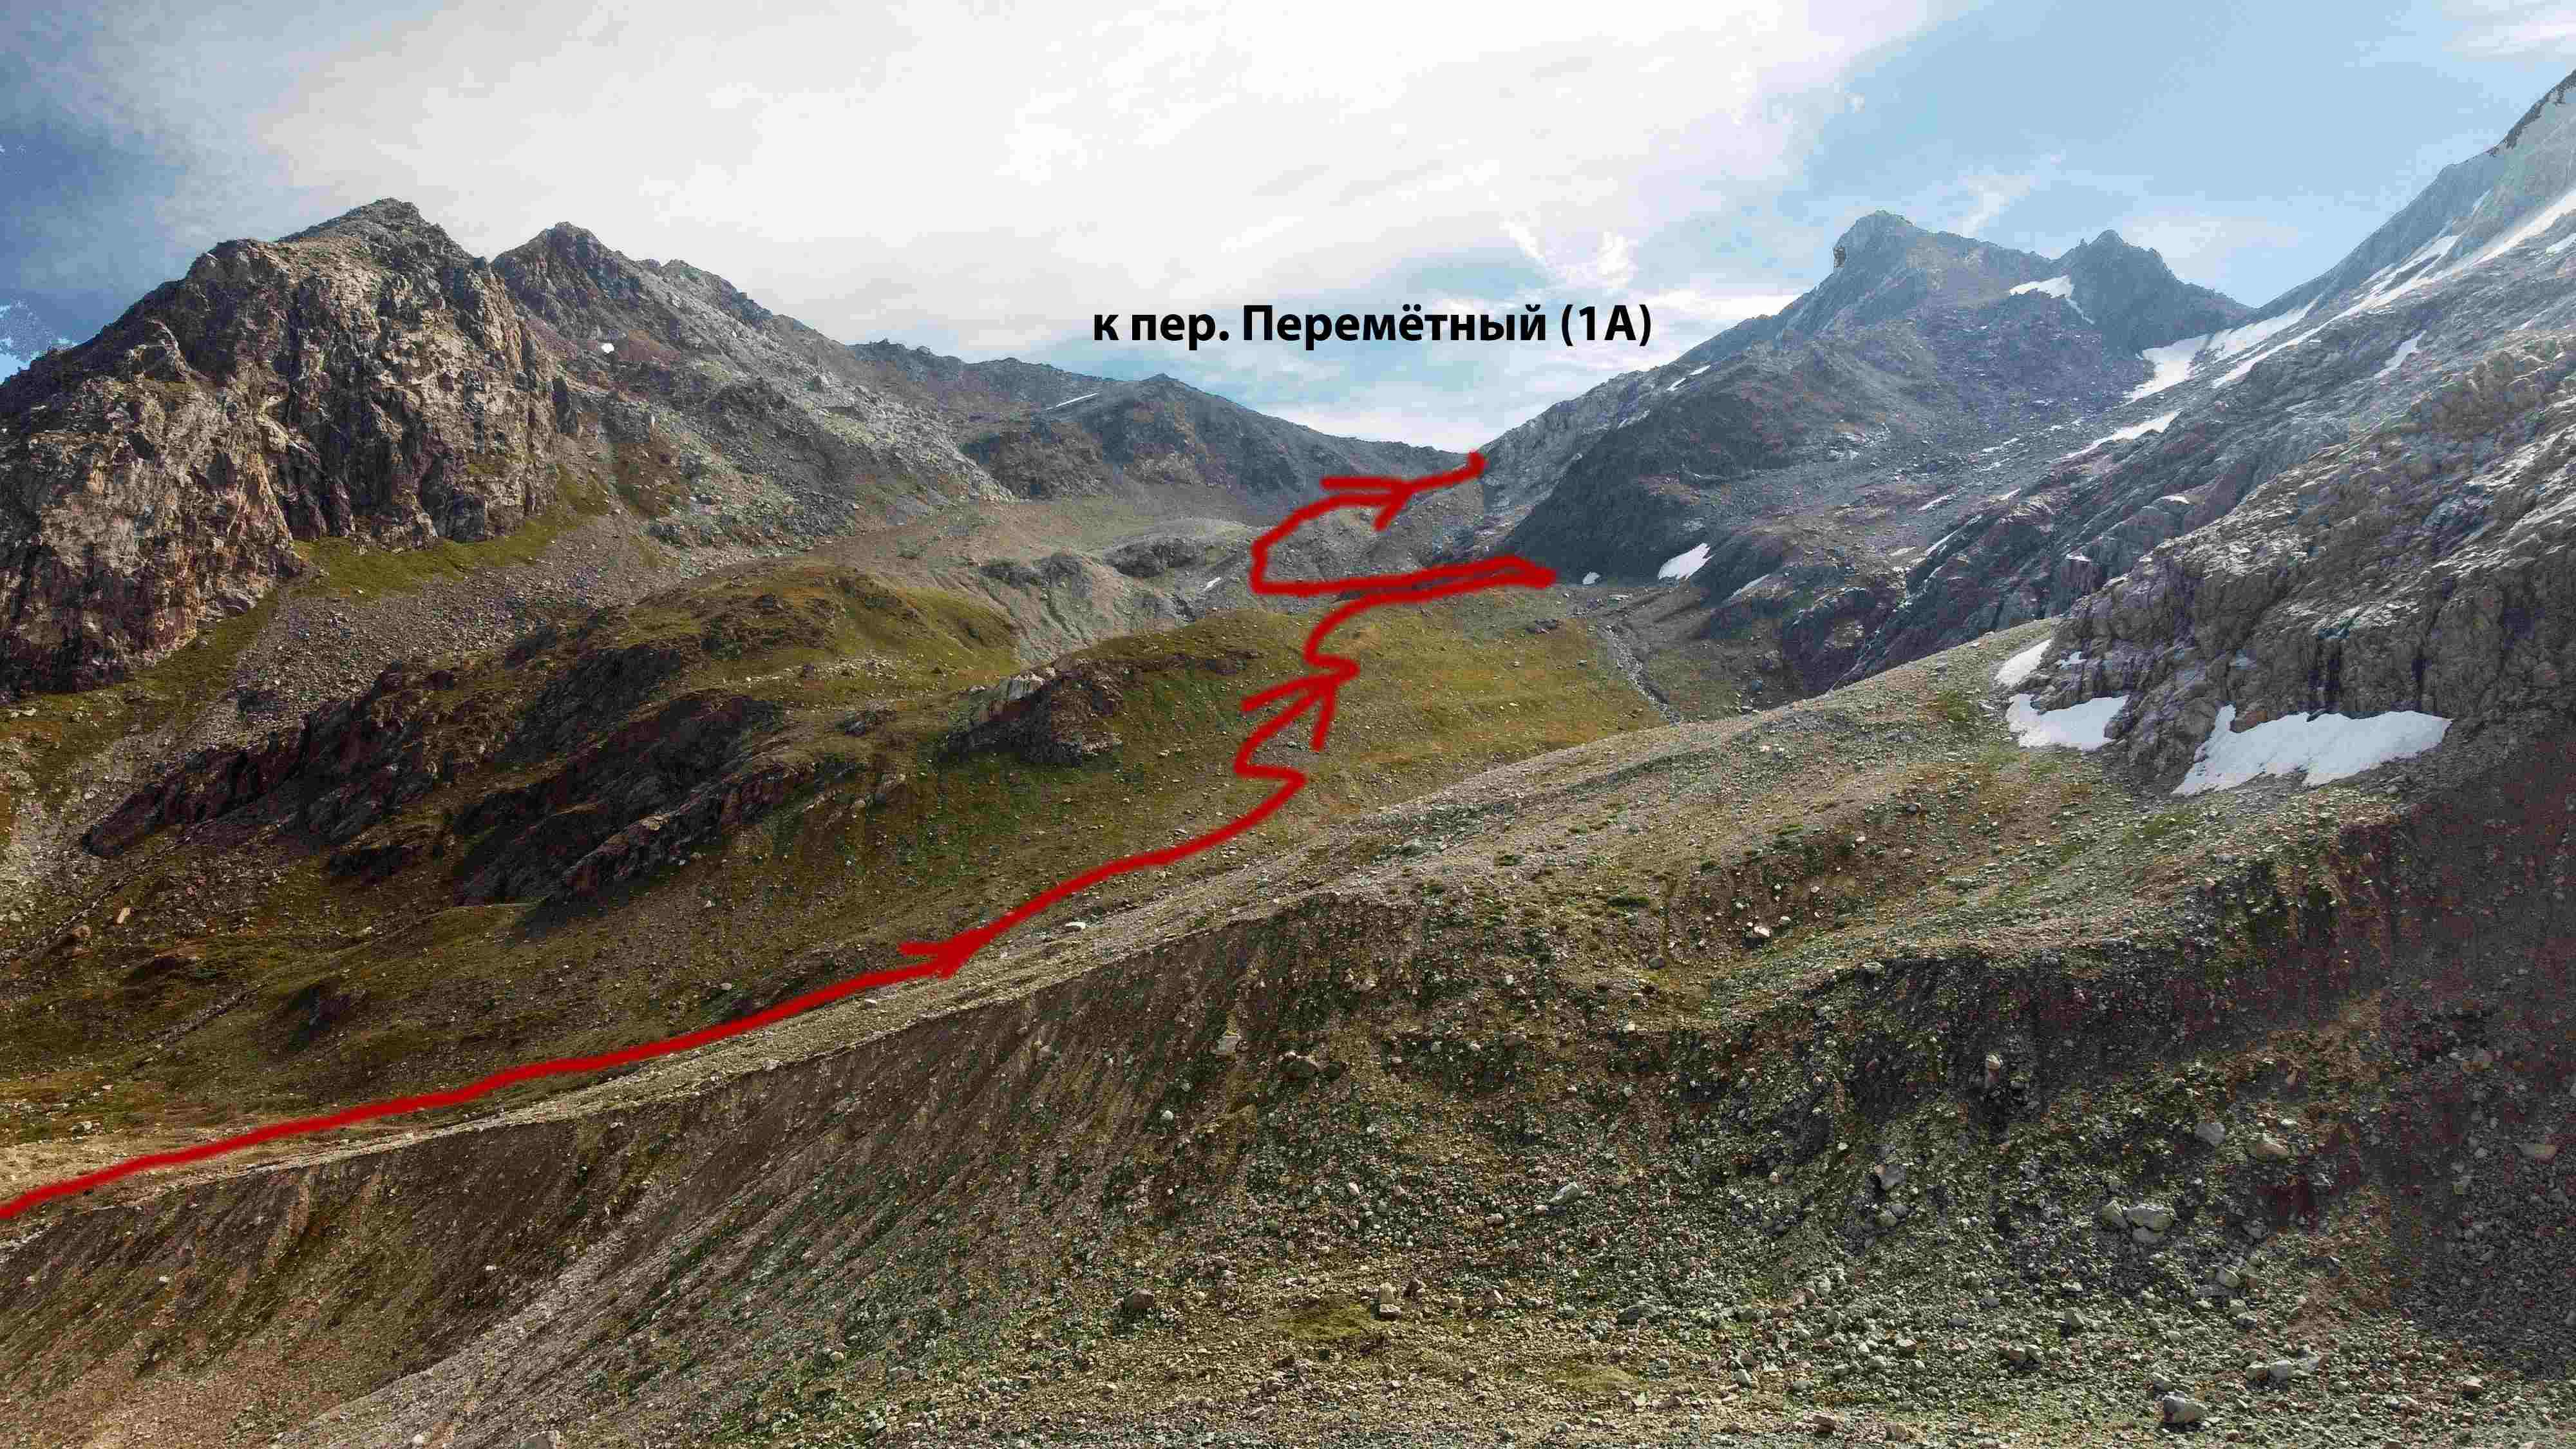
\includegraphics[width=\textwidth]{../pics/perem_1}			
\end{frame}

\begin{frame}
	\frametitle{Траверс по моренам и выход на моренный гребень}
	\framesubtitle{День 10, 27 августа}
	\centering
	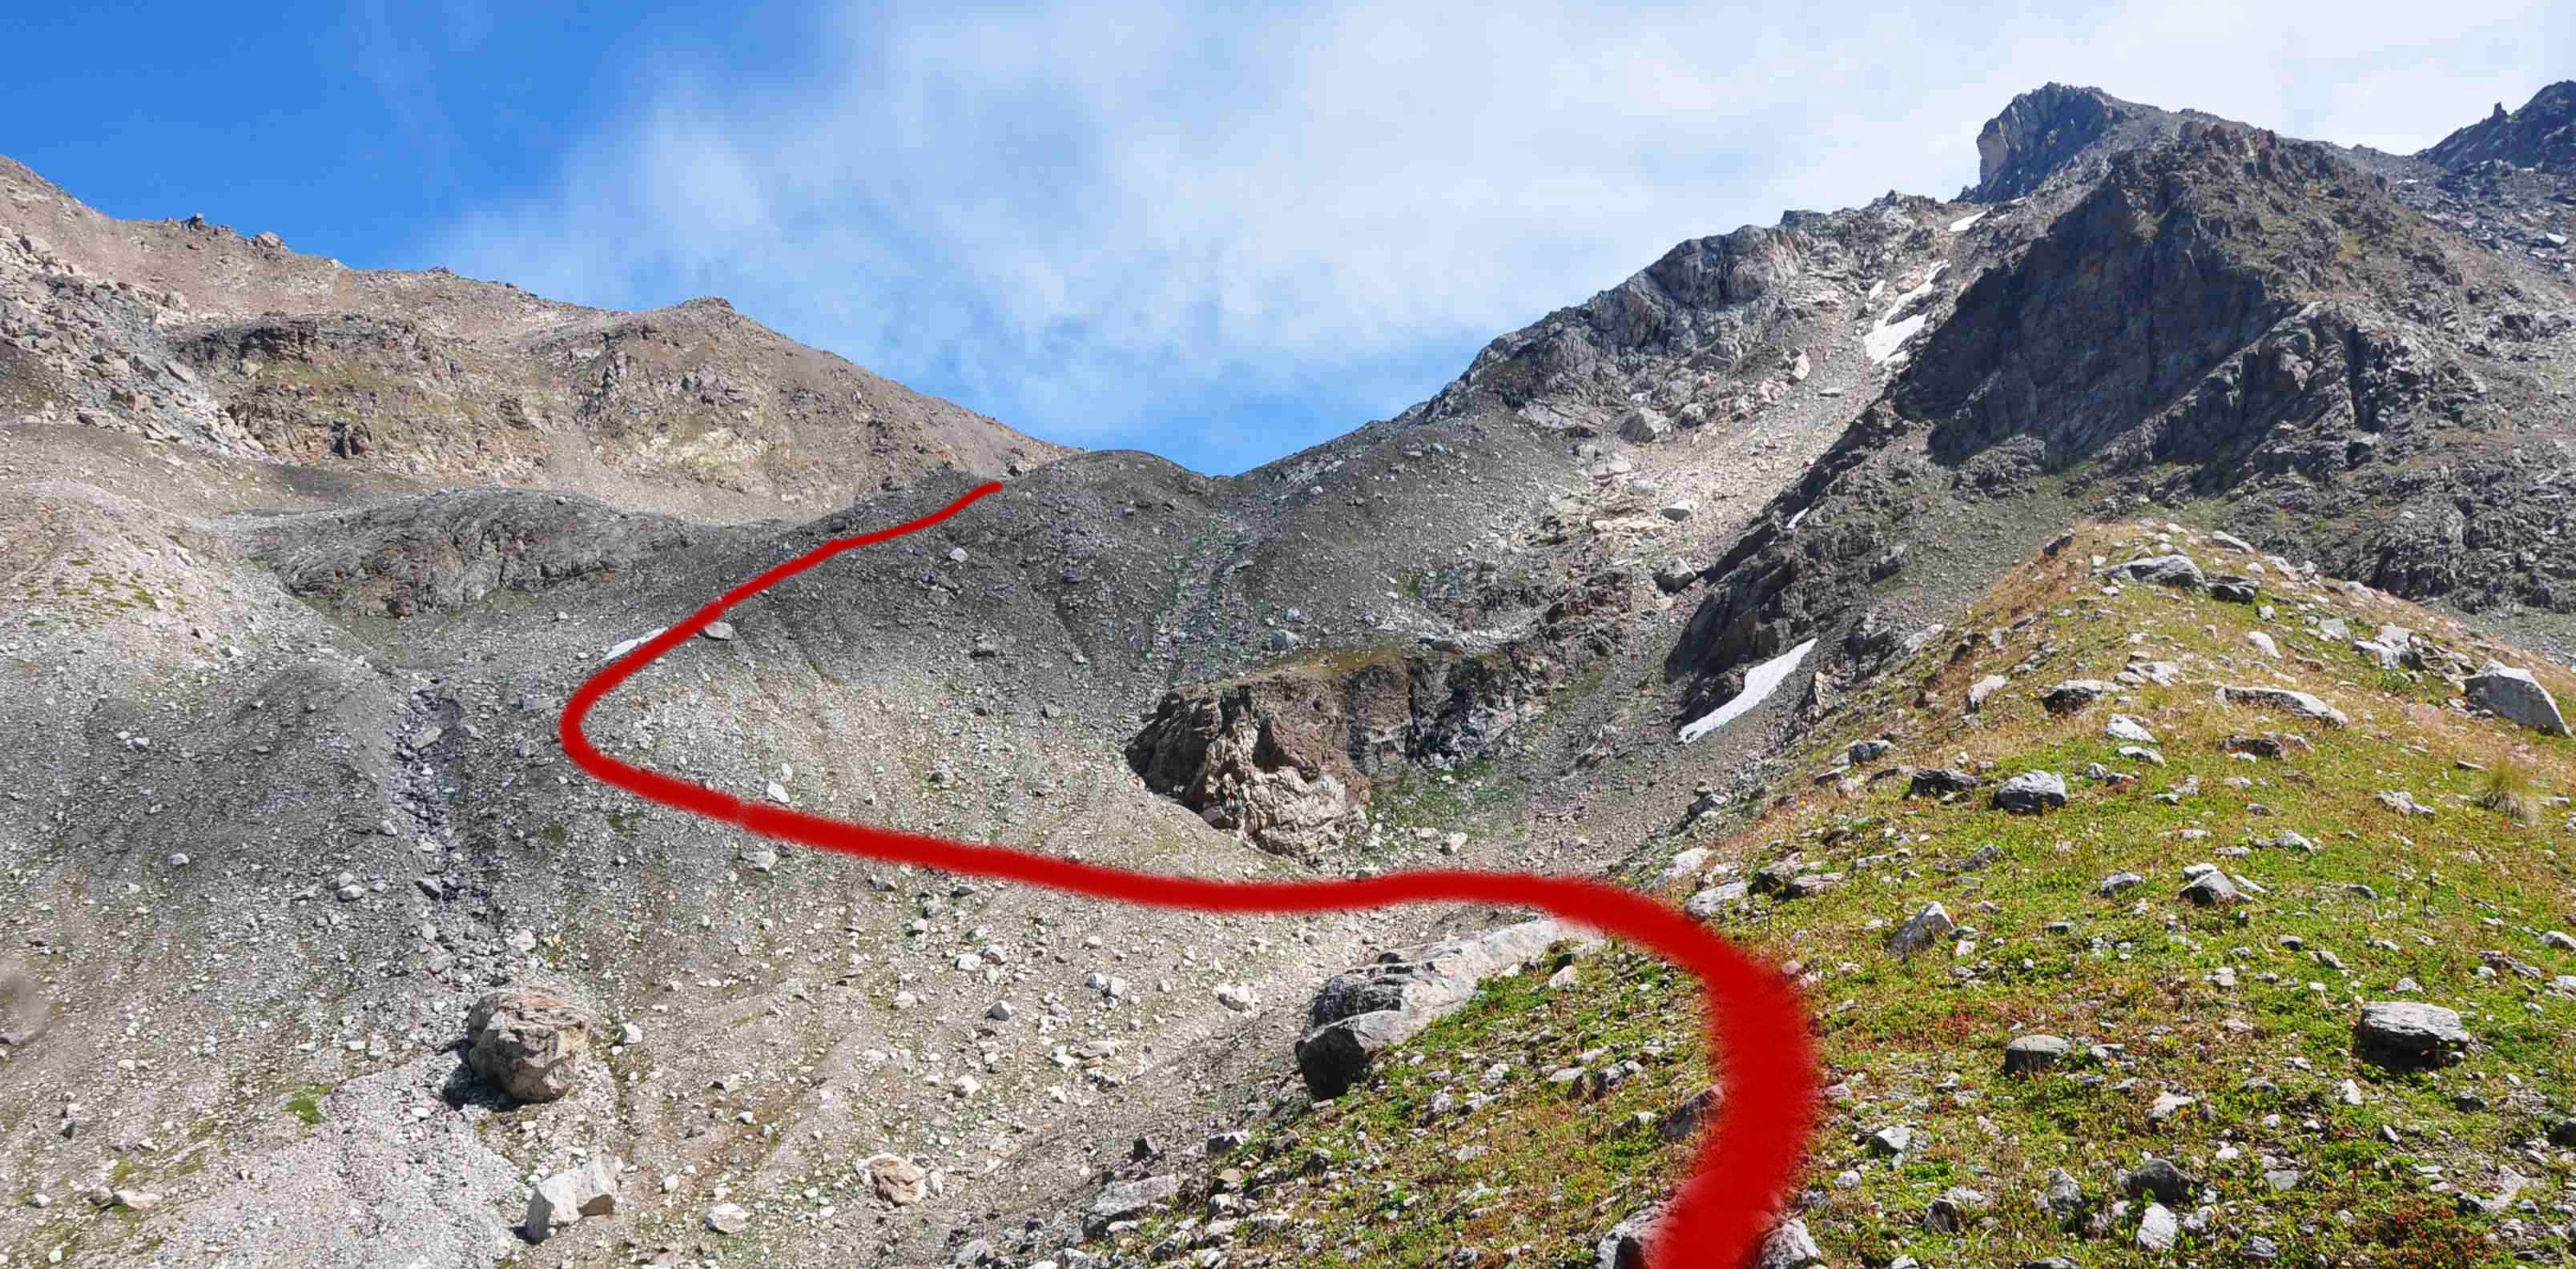
\includegraphics[width=\textwidth]{../pics/DSC_0280}			
\end{frame}

\begin{frame}
	\frametitle{Перевальный взлёт}
	\framesubtitle{День 10, 27 августа}
	\centering
	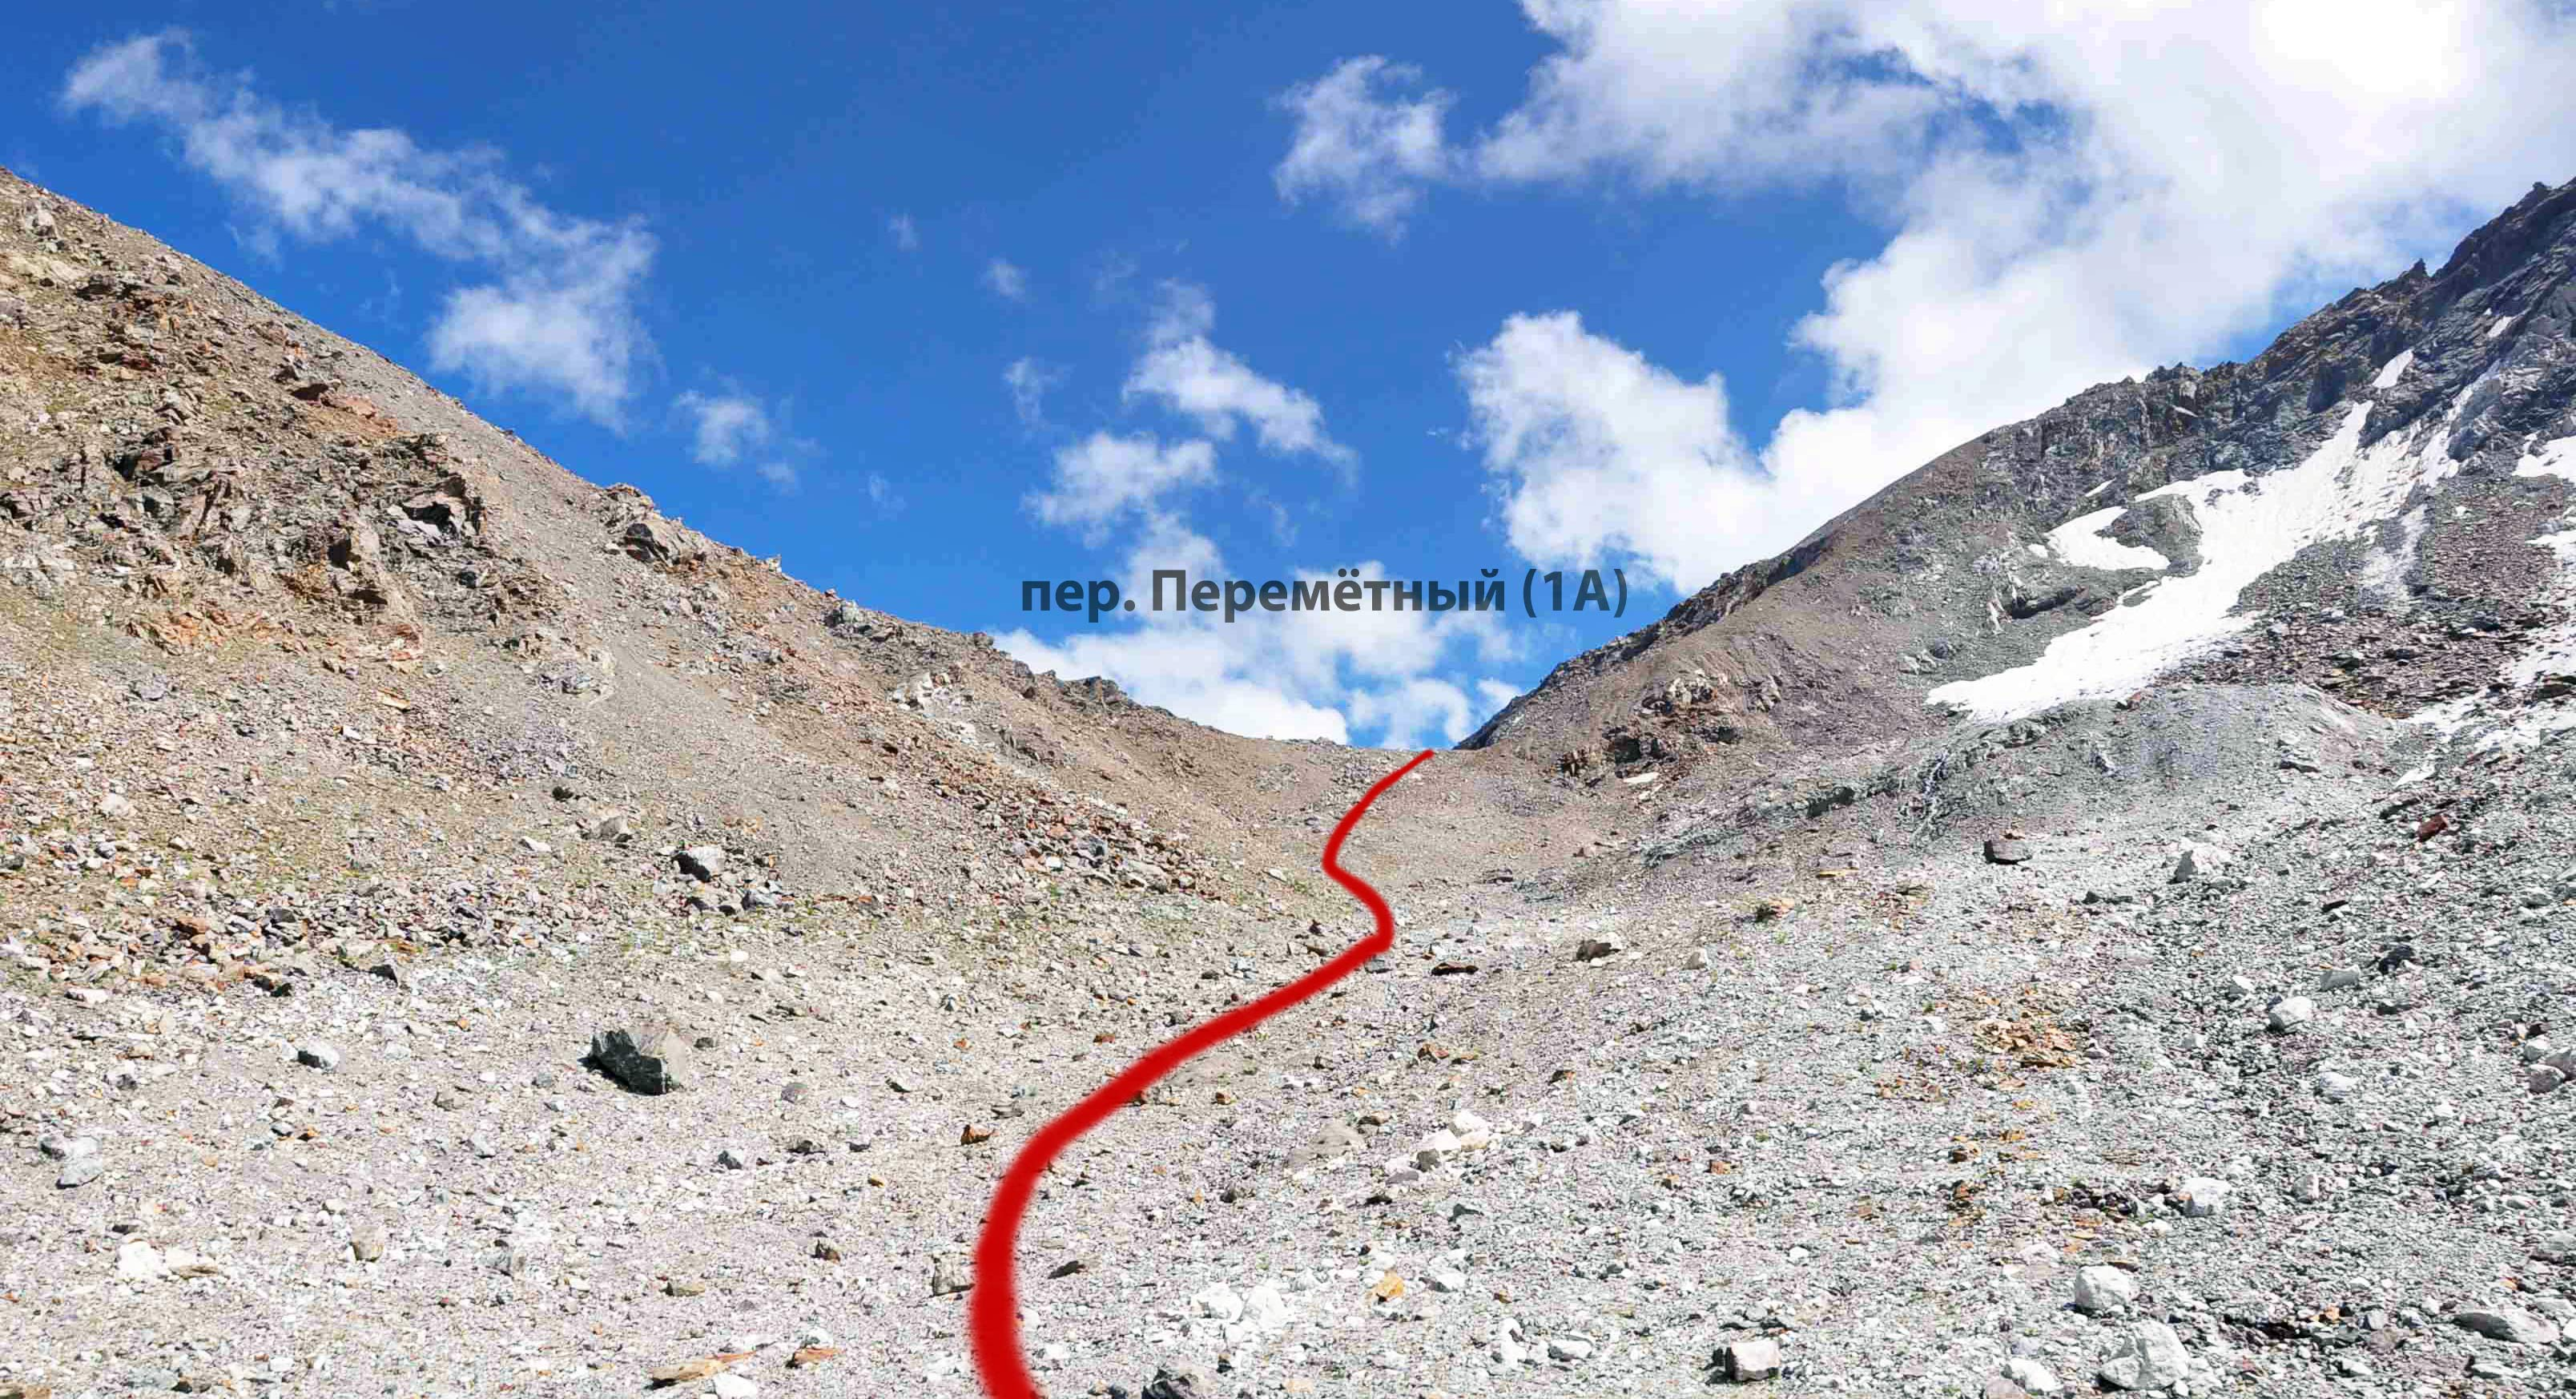
\includegraphics[width=\textwidth]{../pics/DSC_0341}			
\end{frame}

\begin{frame}
	\frametitle{Группа на пер. Перемётный (1А)}
	\framesubtitle{День 10, 27 августа}
	{\tiny
		\begin{minipage}{\fourpicsize}
			\centering
			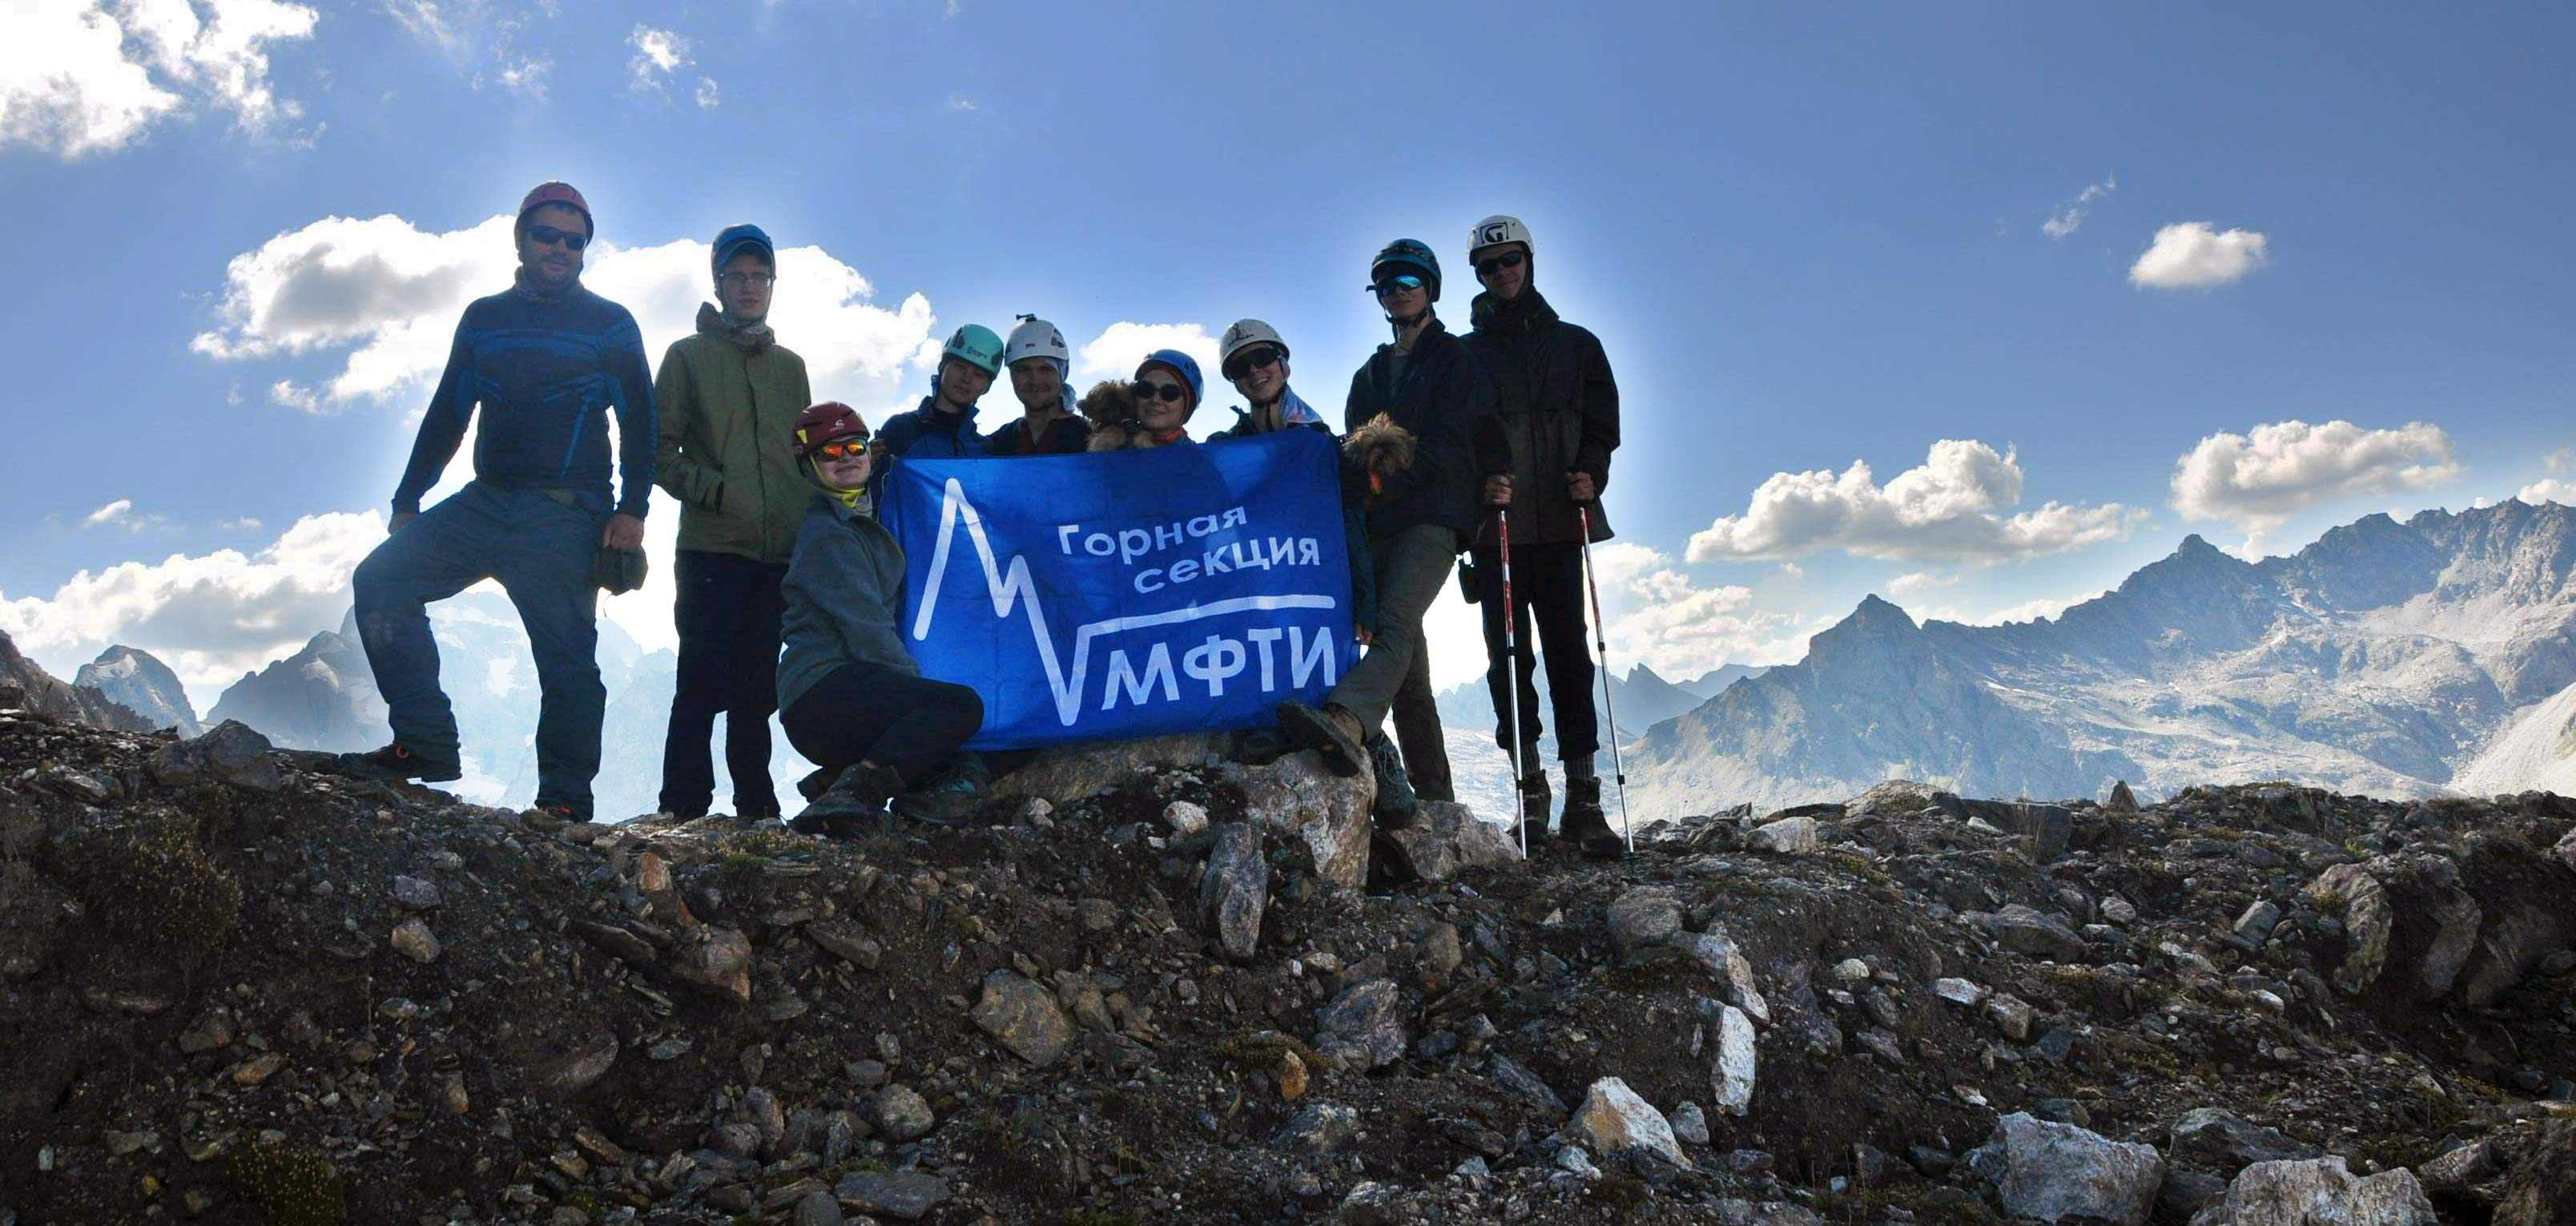
\includegraphics[width=\textwidth]{../pics/DSC_0412 2.jpg}			
			Вид в д.р. Чунгур-Джар
		\end{minipage}
		\hfill
		\begin{minipage}{\fourpicsize}
			\centering
			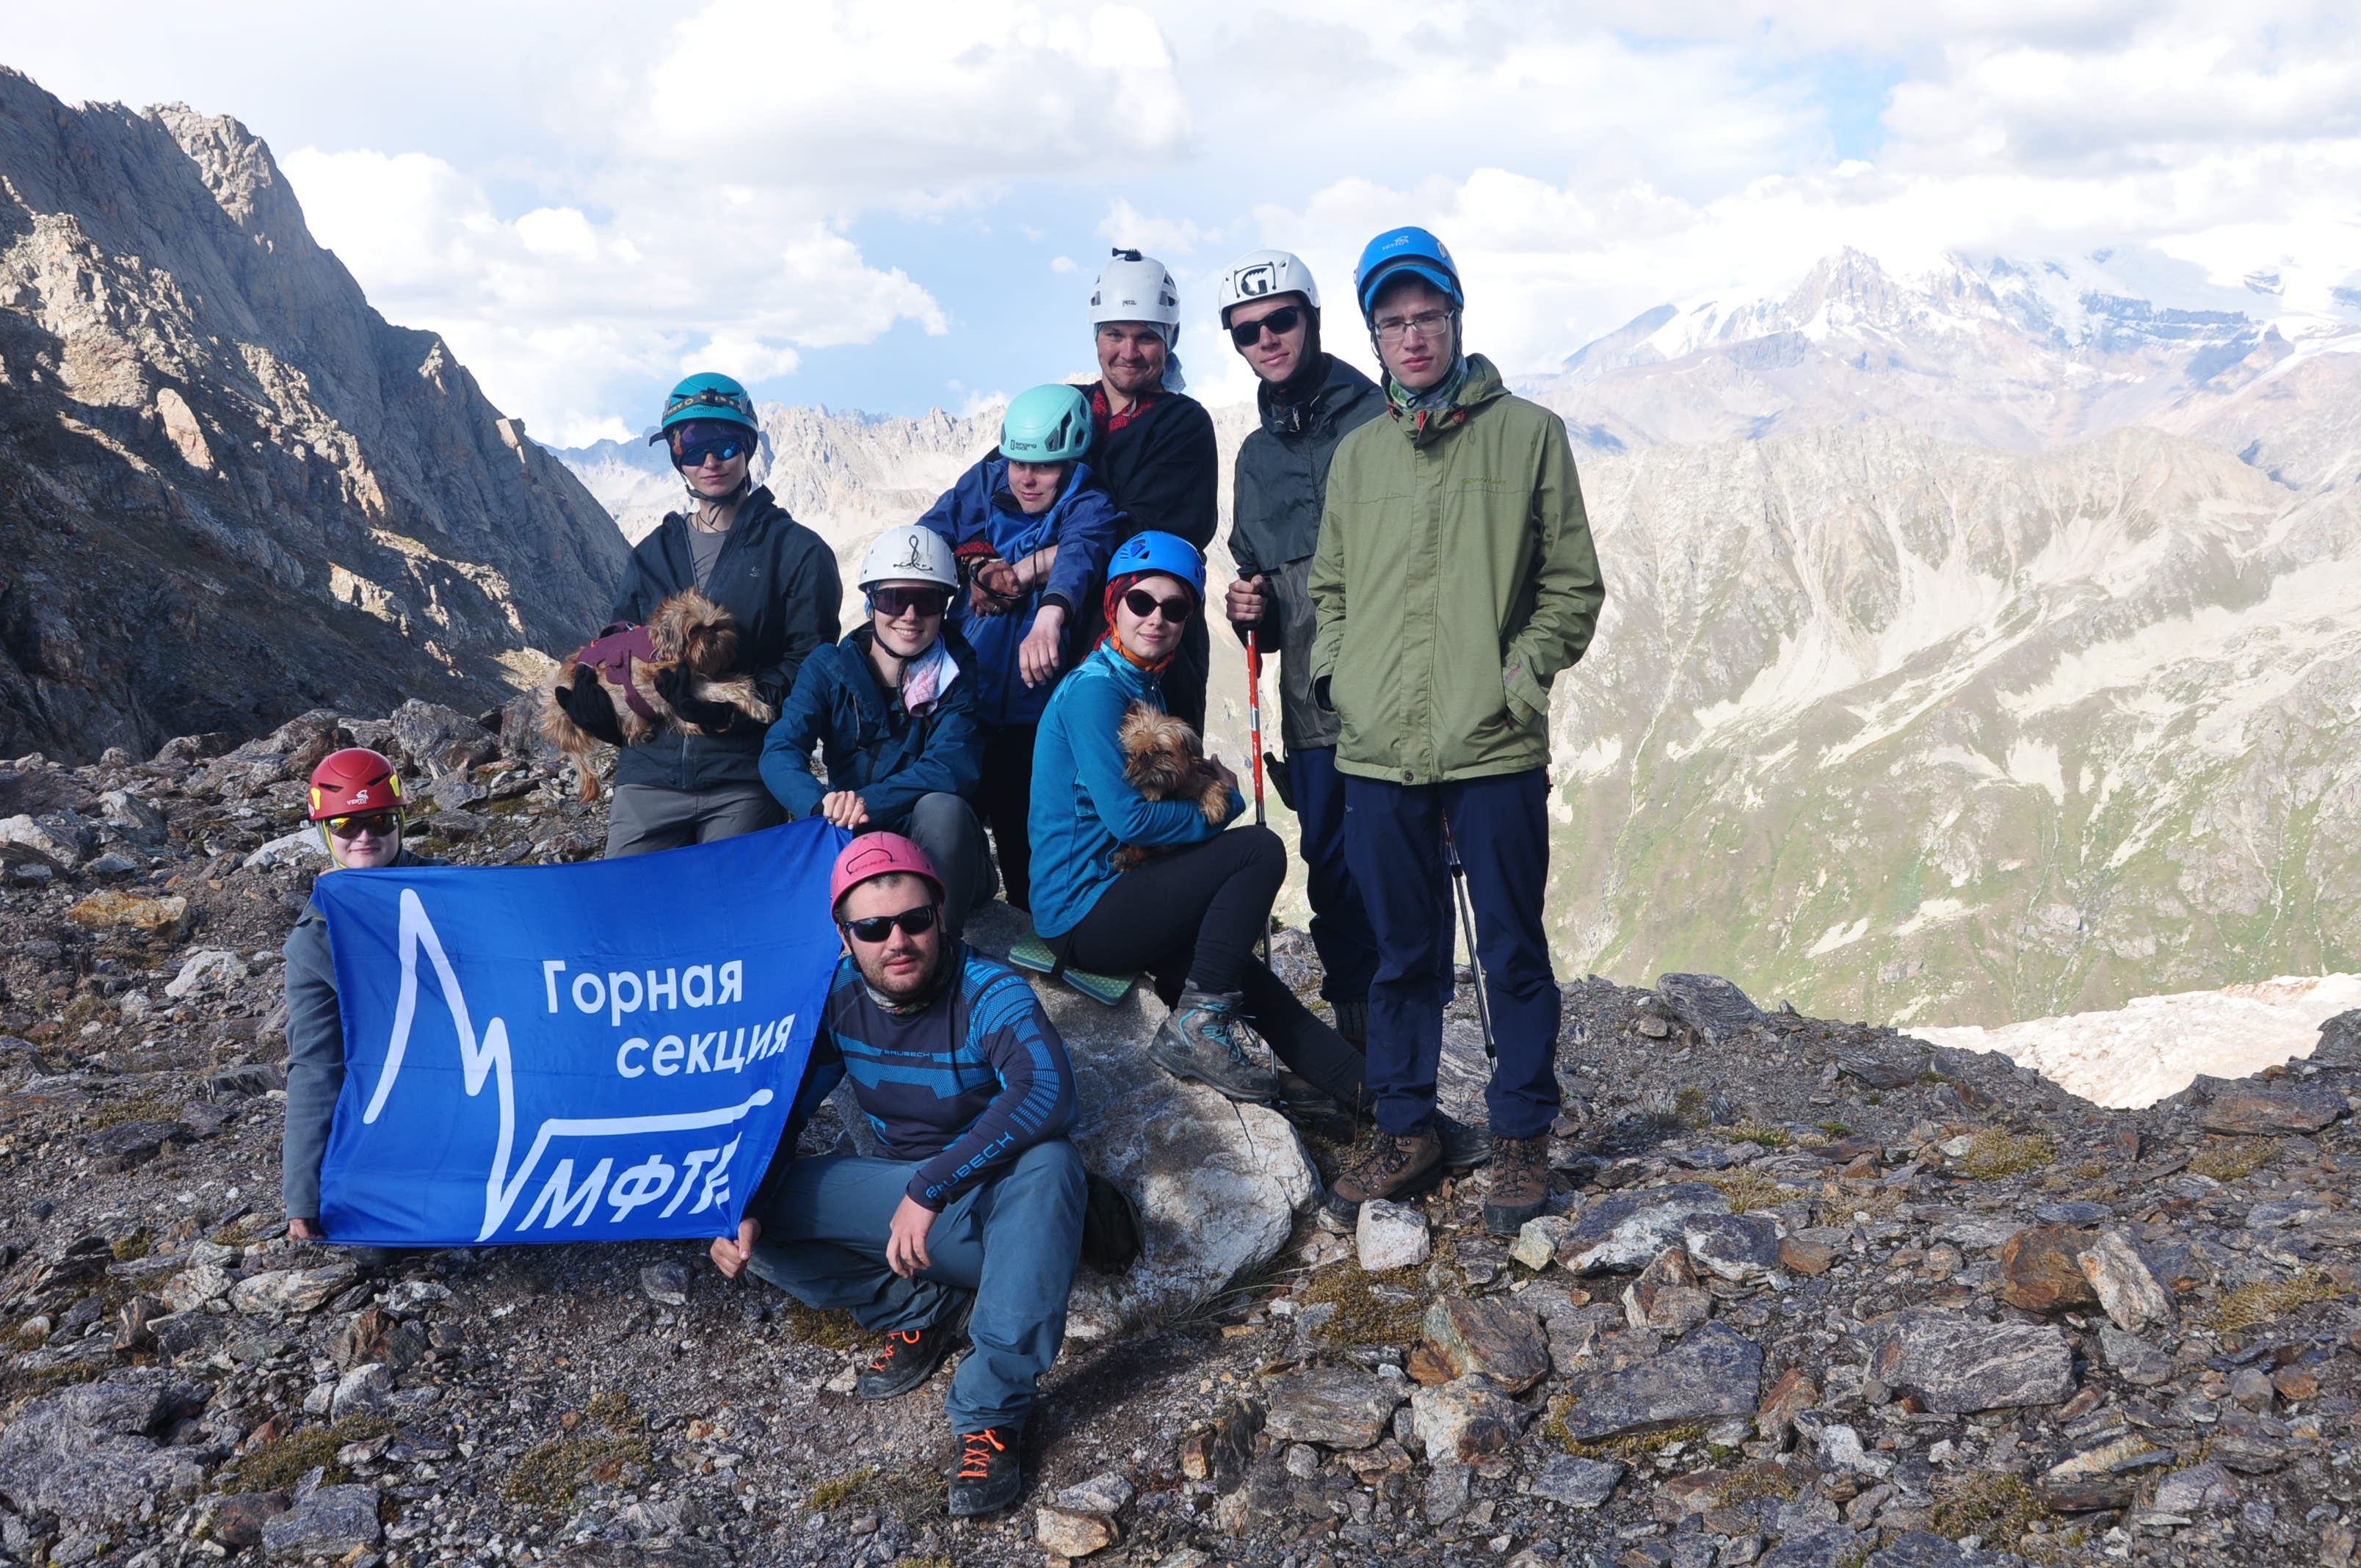
\includegraphics[width=\textwidth]{../pics/DSC_0419 2.jpg}			
			Вид в д.р. Танышхан
		\end{minipage}
		\vfill
	}
\end{frame}

\begin{frame}
	\frametitle{Фотоньки с перевала}
	\framesubtitle{День 10, 27 августа}
	\centering
	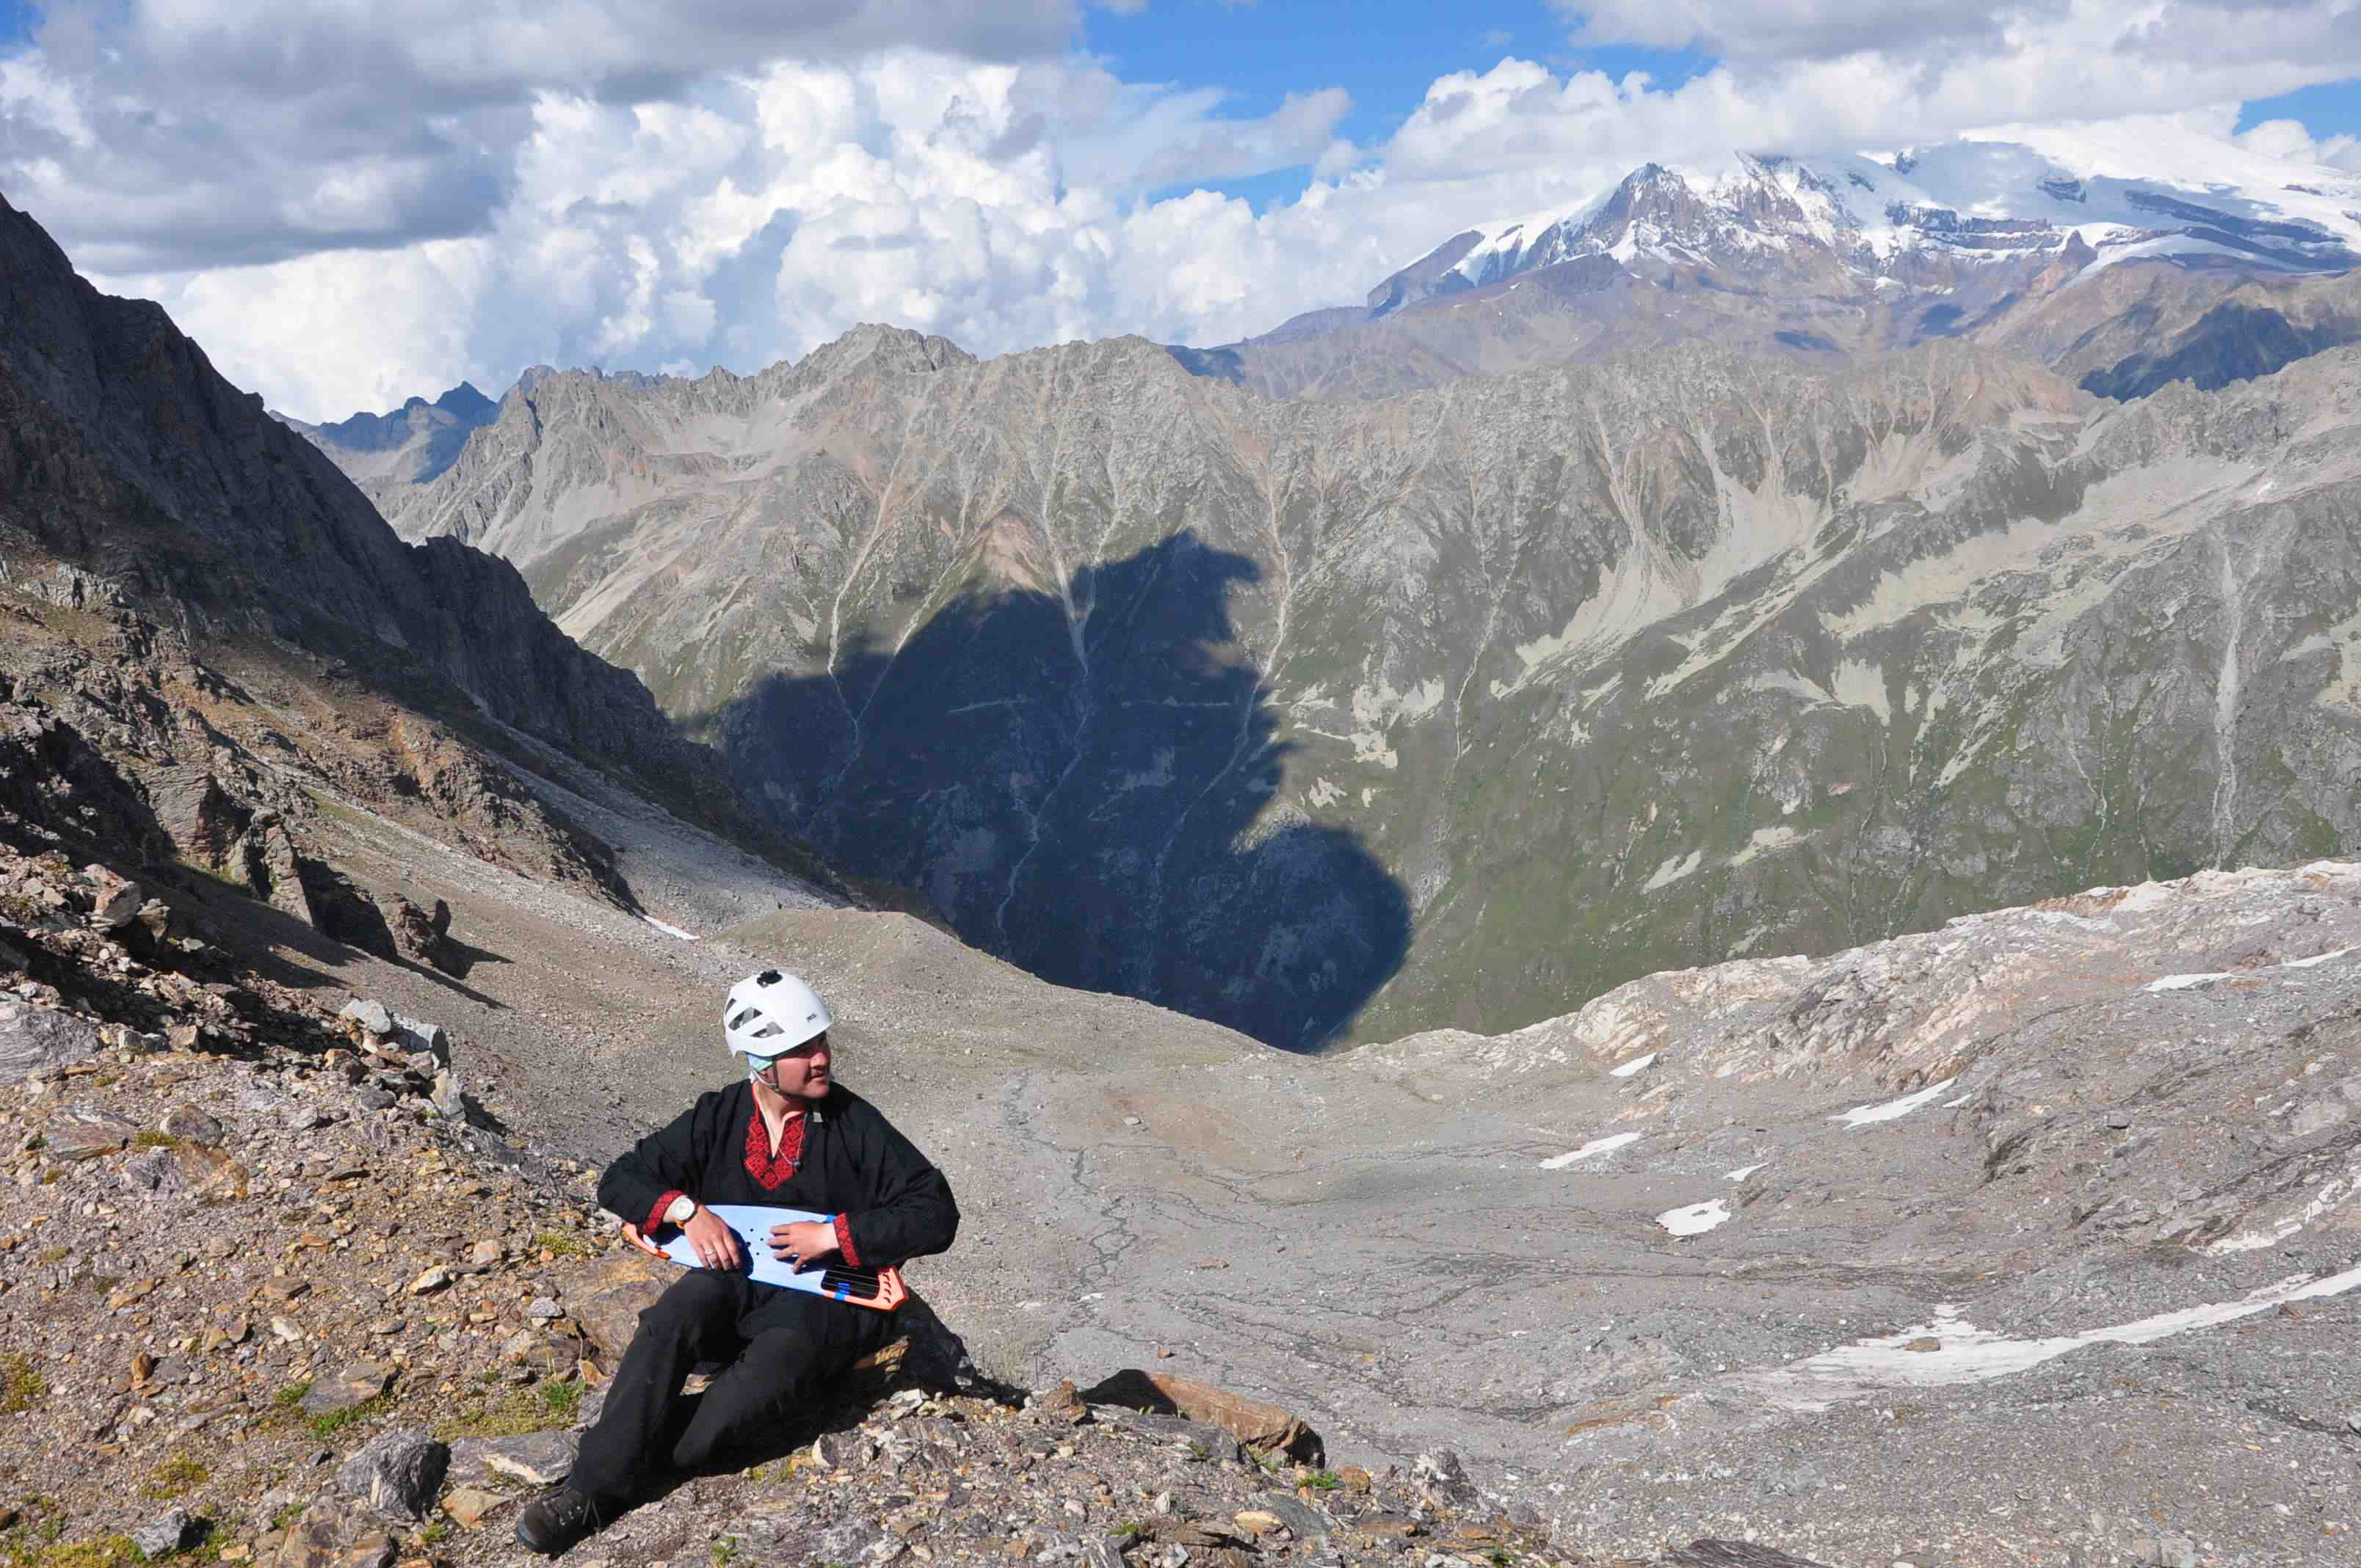
\includegraphics[width=\textwidth]{../pics/DSC_0369 2}			
\end{frame}

\begin{frame}
	\frametitle{Фотоньки с перевала}
	\framesubtitle{День 10, 27 августа}
	\centering
	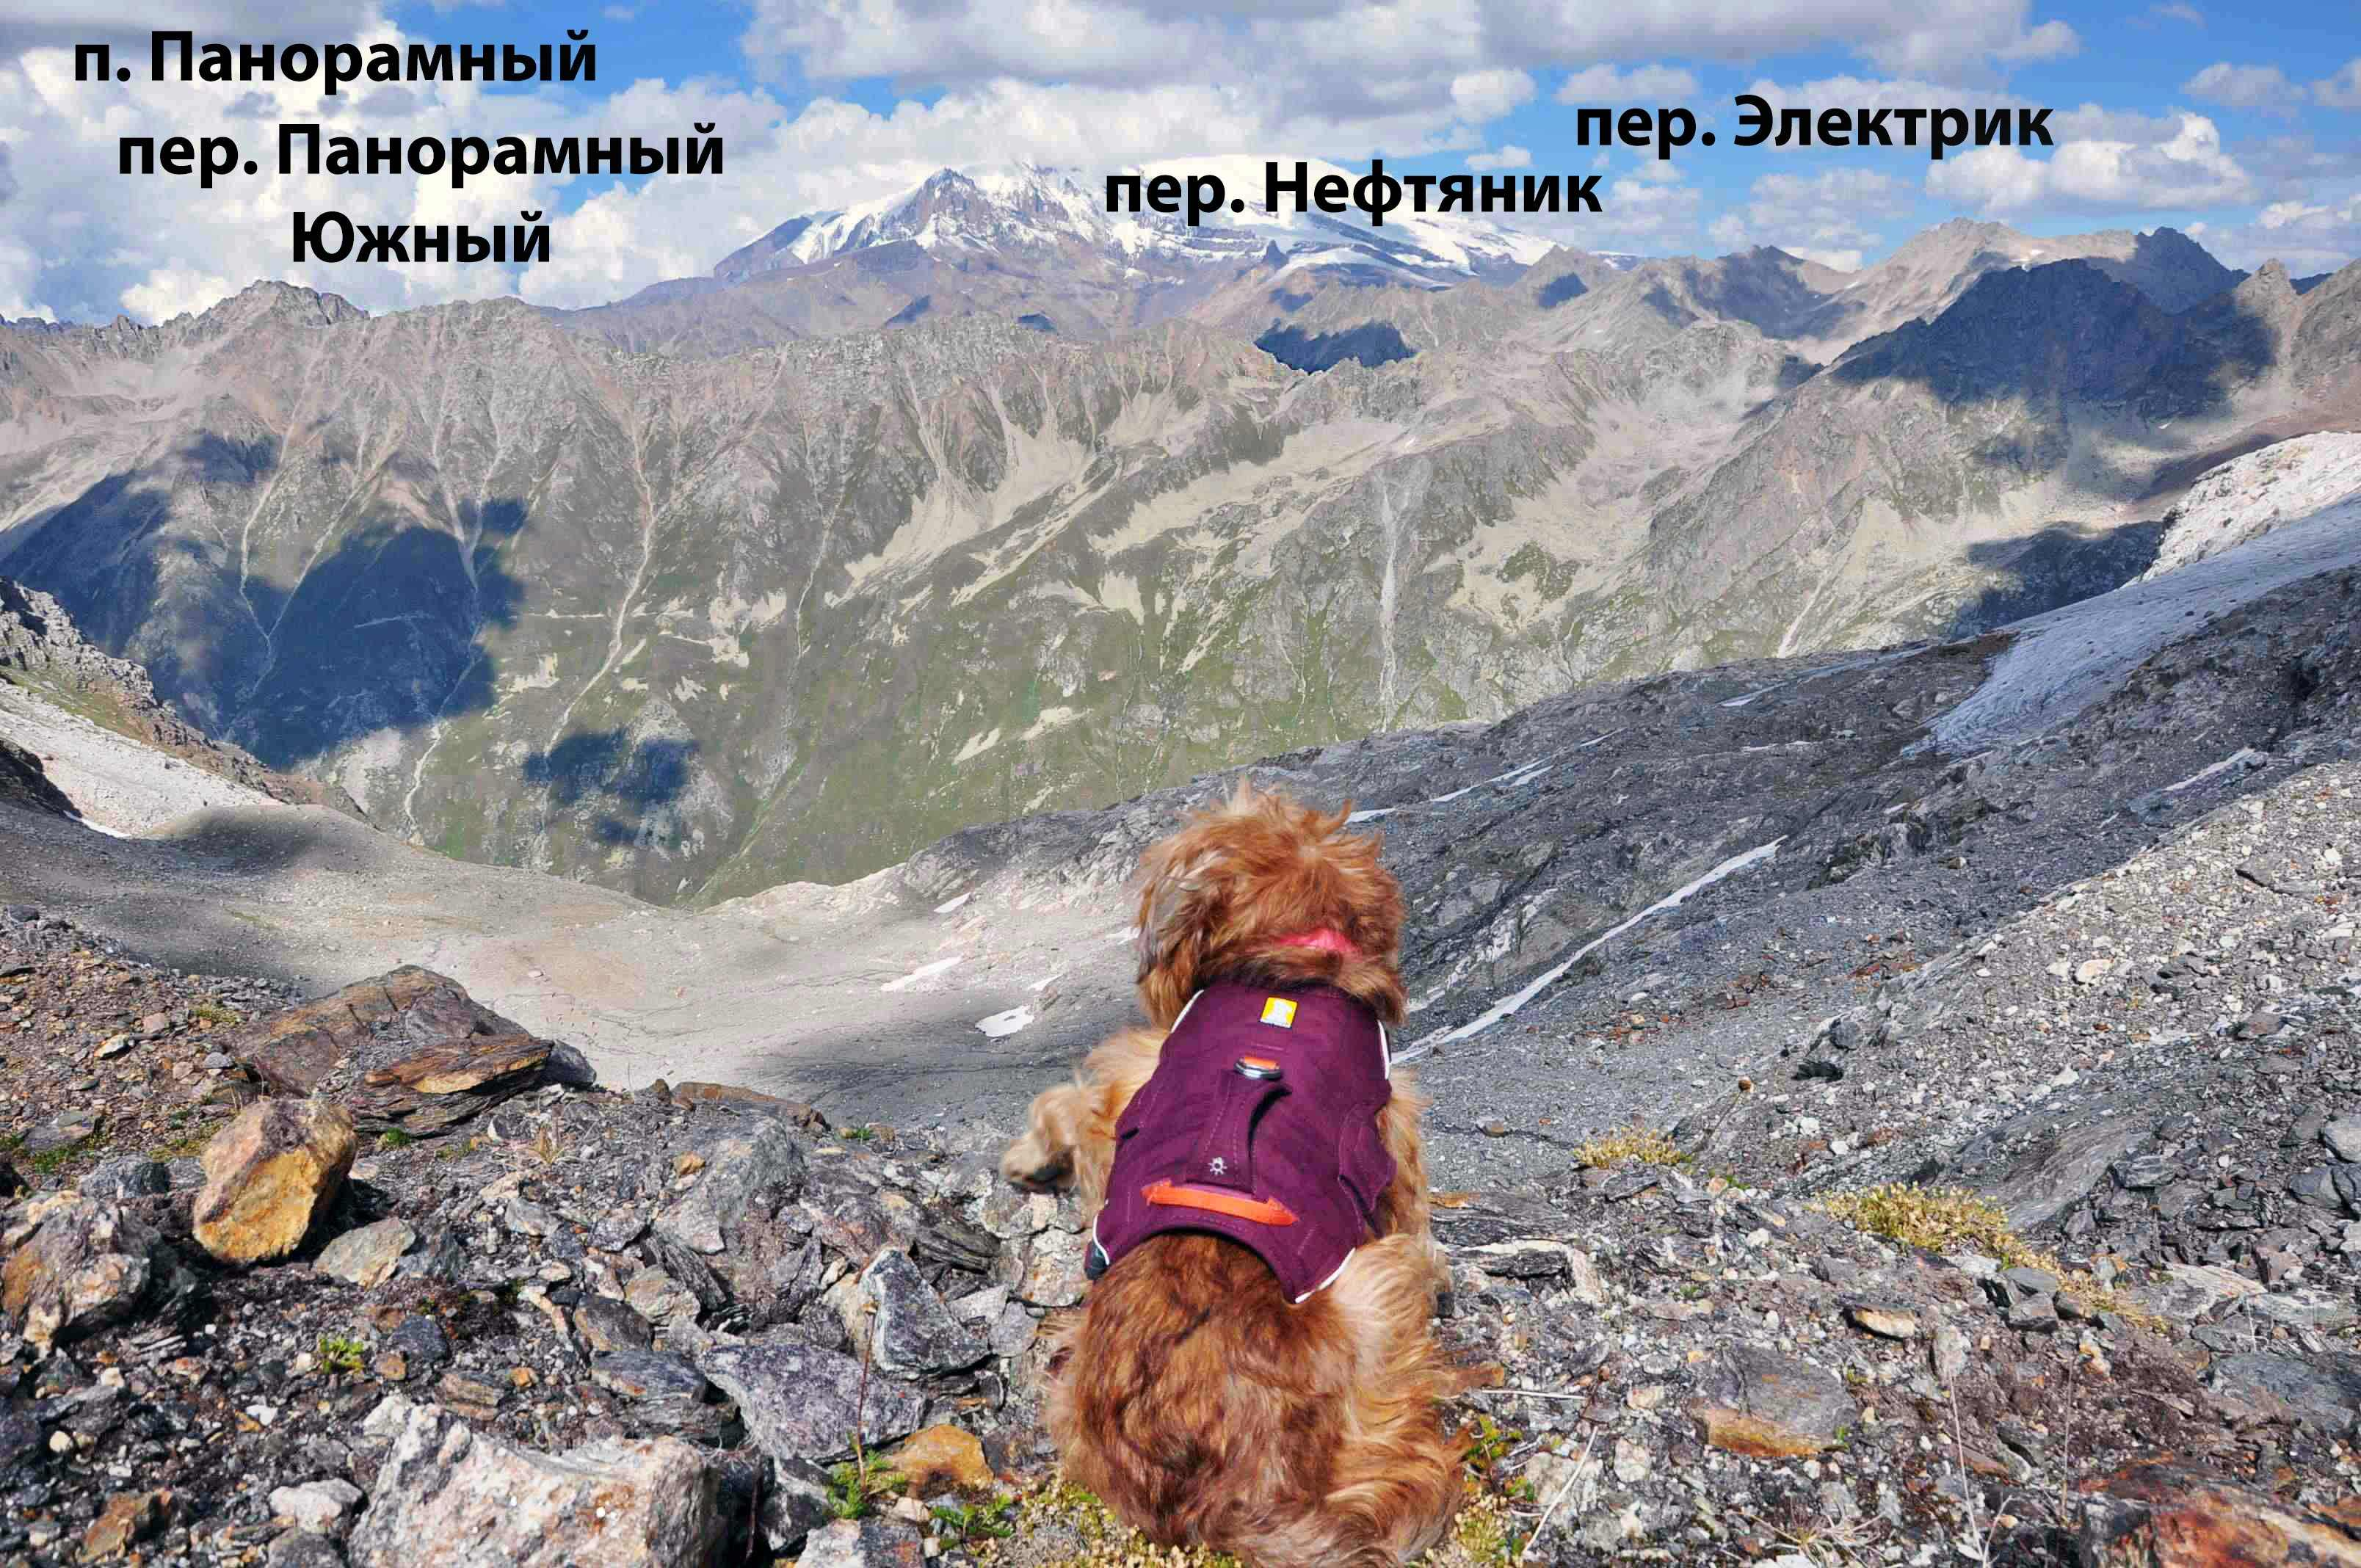
\includegraphics[width=\textwidth]{../pics/DSC_0385 2}			
\end{frame}


\begin{frame}
	\frametitle{Готовность к спуску}
	\framesubtitle{День 10, 27 августа}
	\centering
	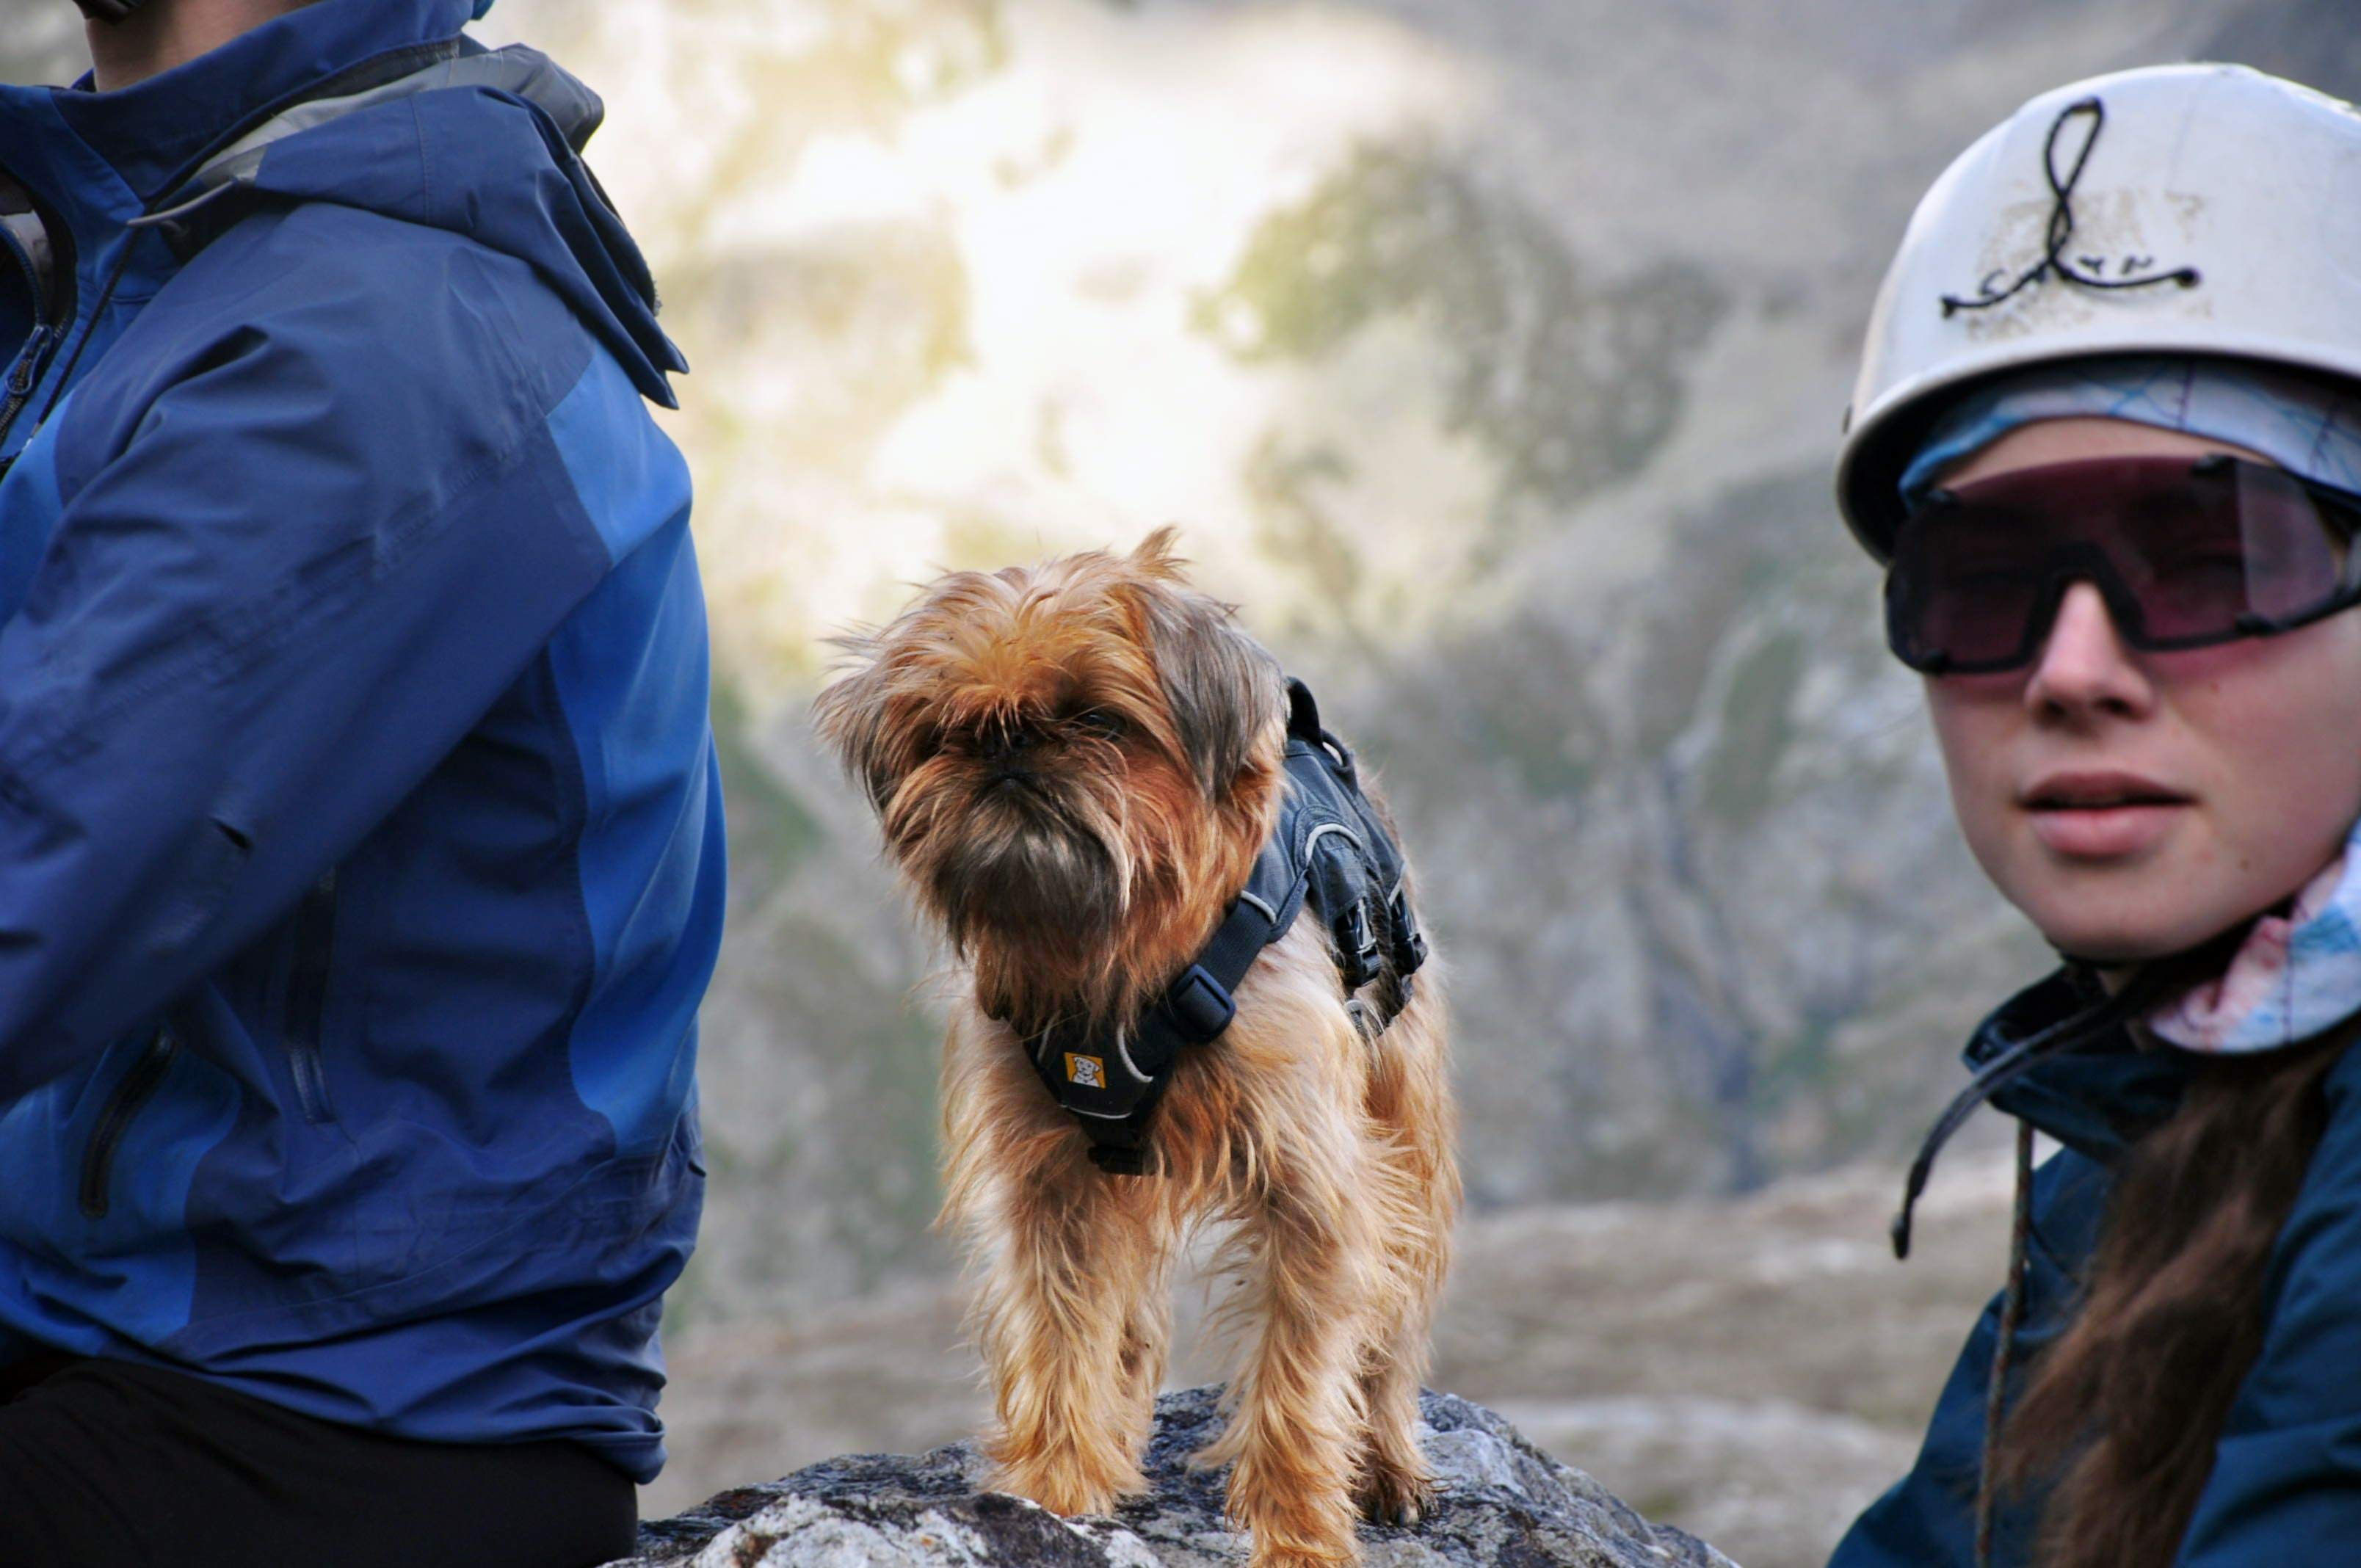
\includegraphics[width=\textwidth]{../pics/DSC_0428 2}			
\end{frame}

\begin{frame}
	\frametitle{Спуск к «анучинским» ночёвкам на 2900 м}
	\framesubtitle{День 10, 27 августа}
	\centering
	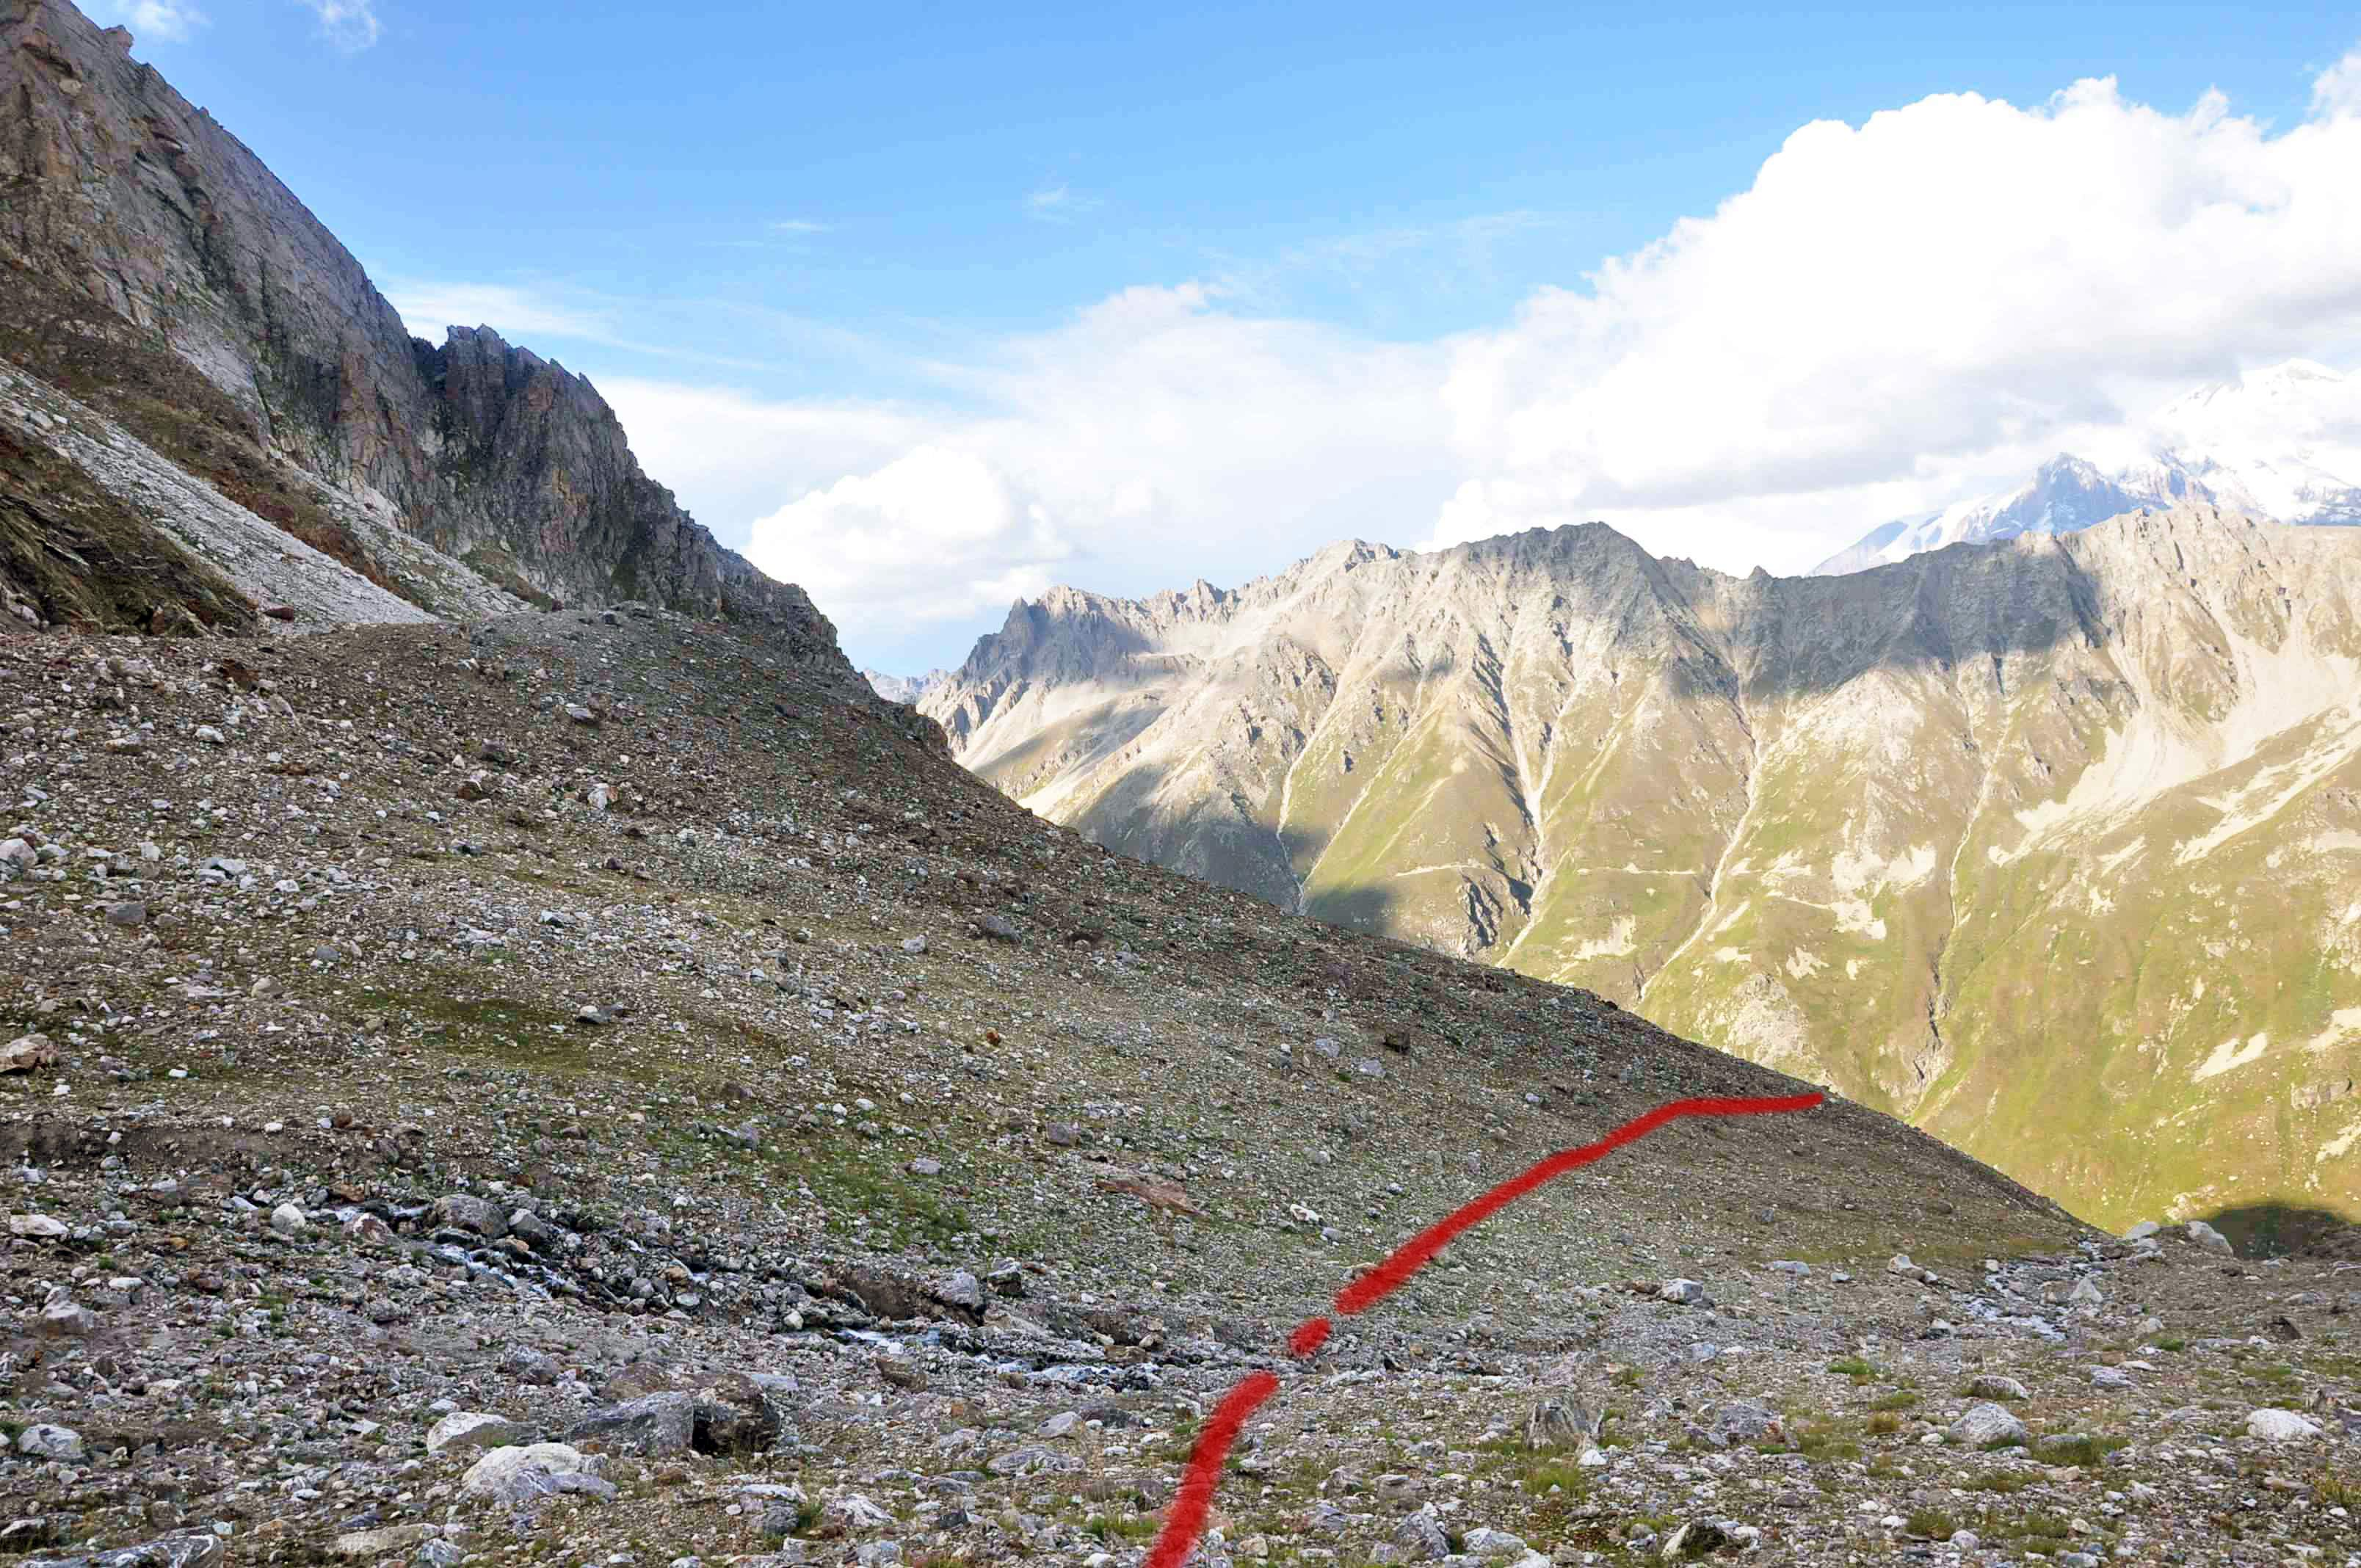
\includegraphics[width=\textwidth]{../pics/DSC_0425 2}			
\end{frame}

\begin{frame}
	\frametitle{Спуск к «анучинским» ночёвкам на 2900 м}
	\framesubtitle{День 10, 27 августа}
	\centering
	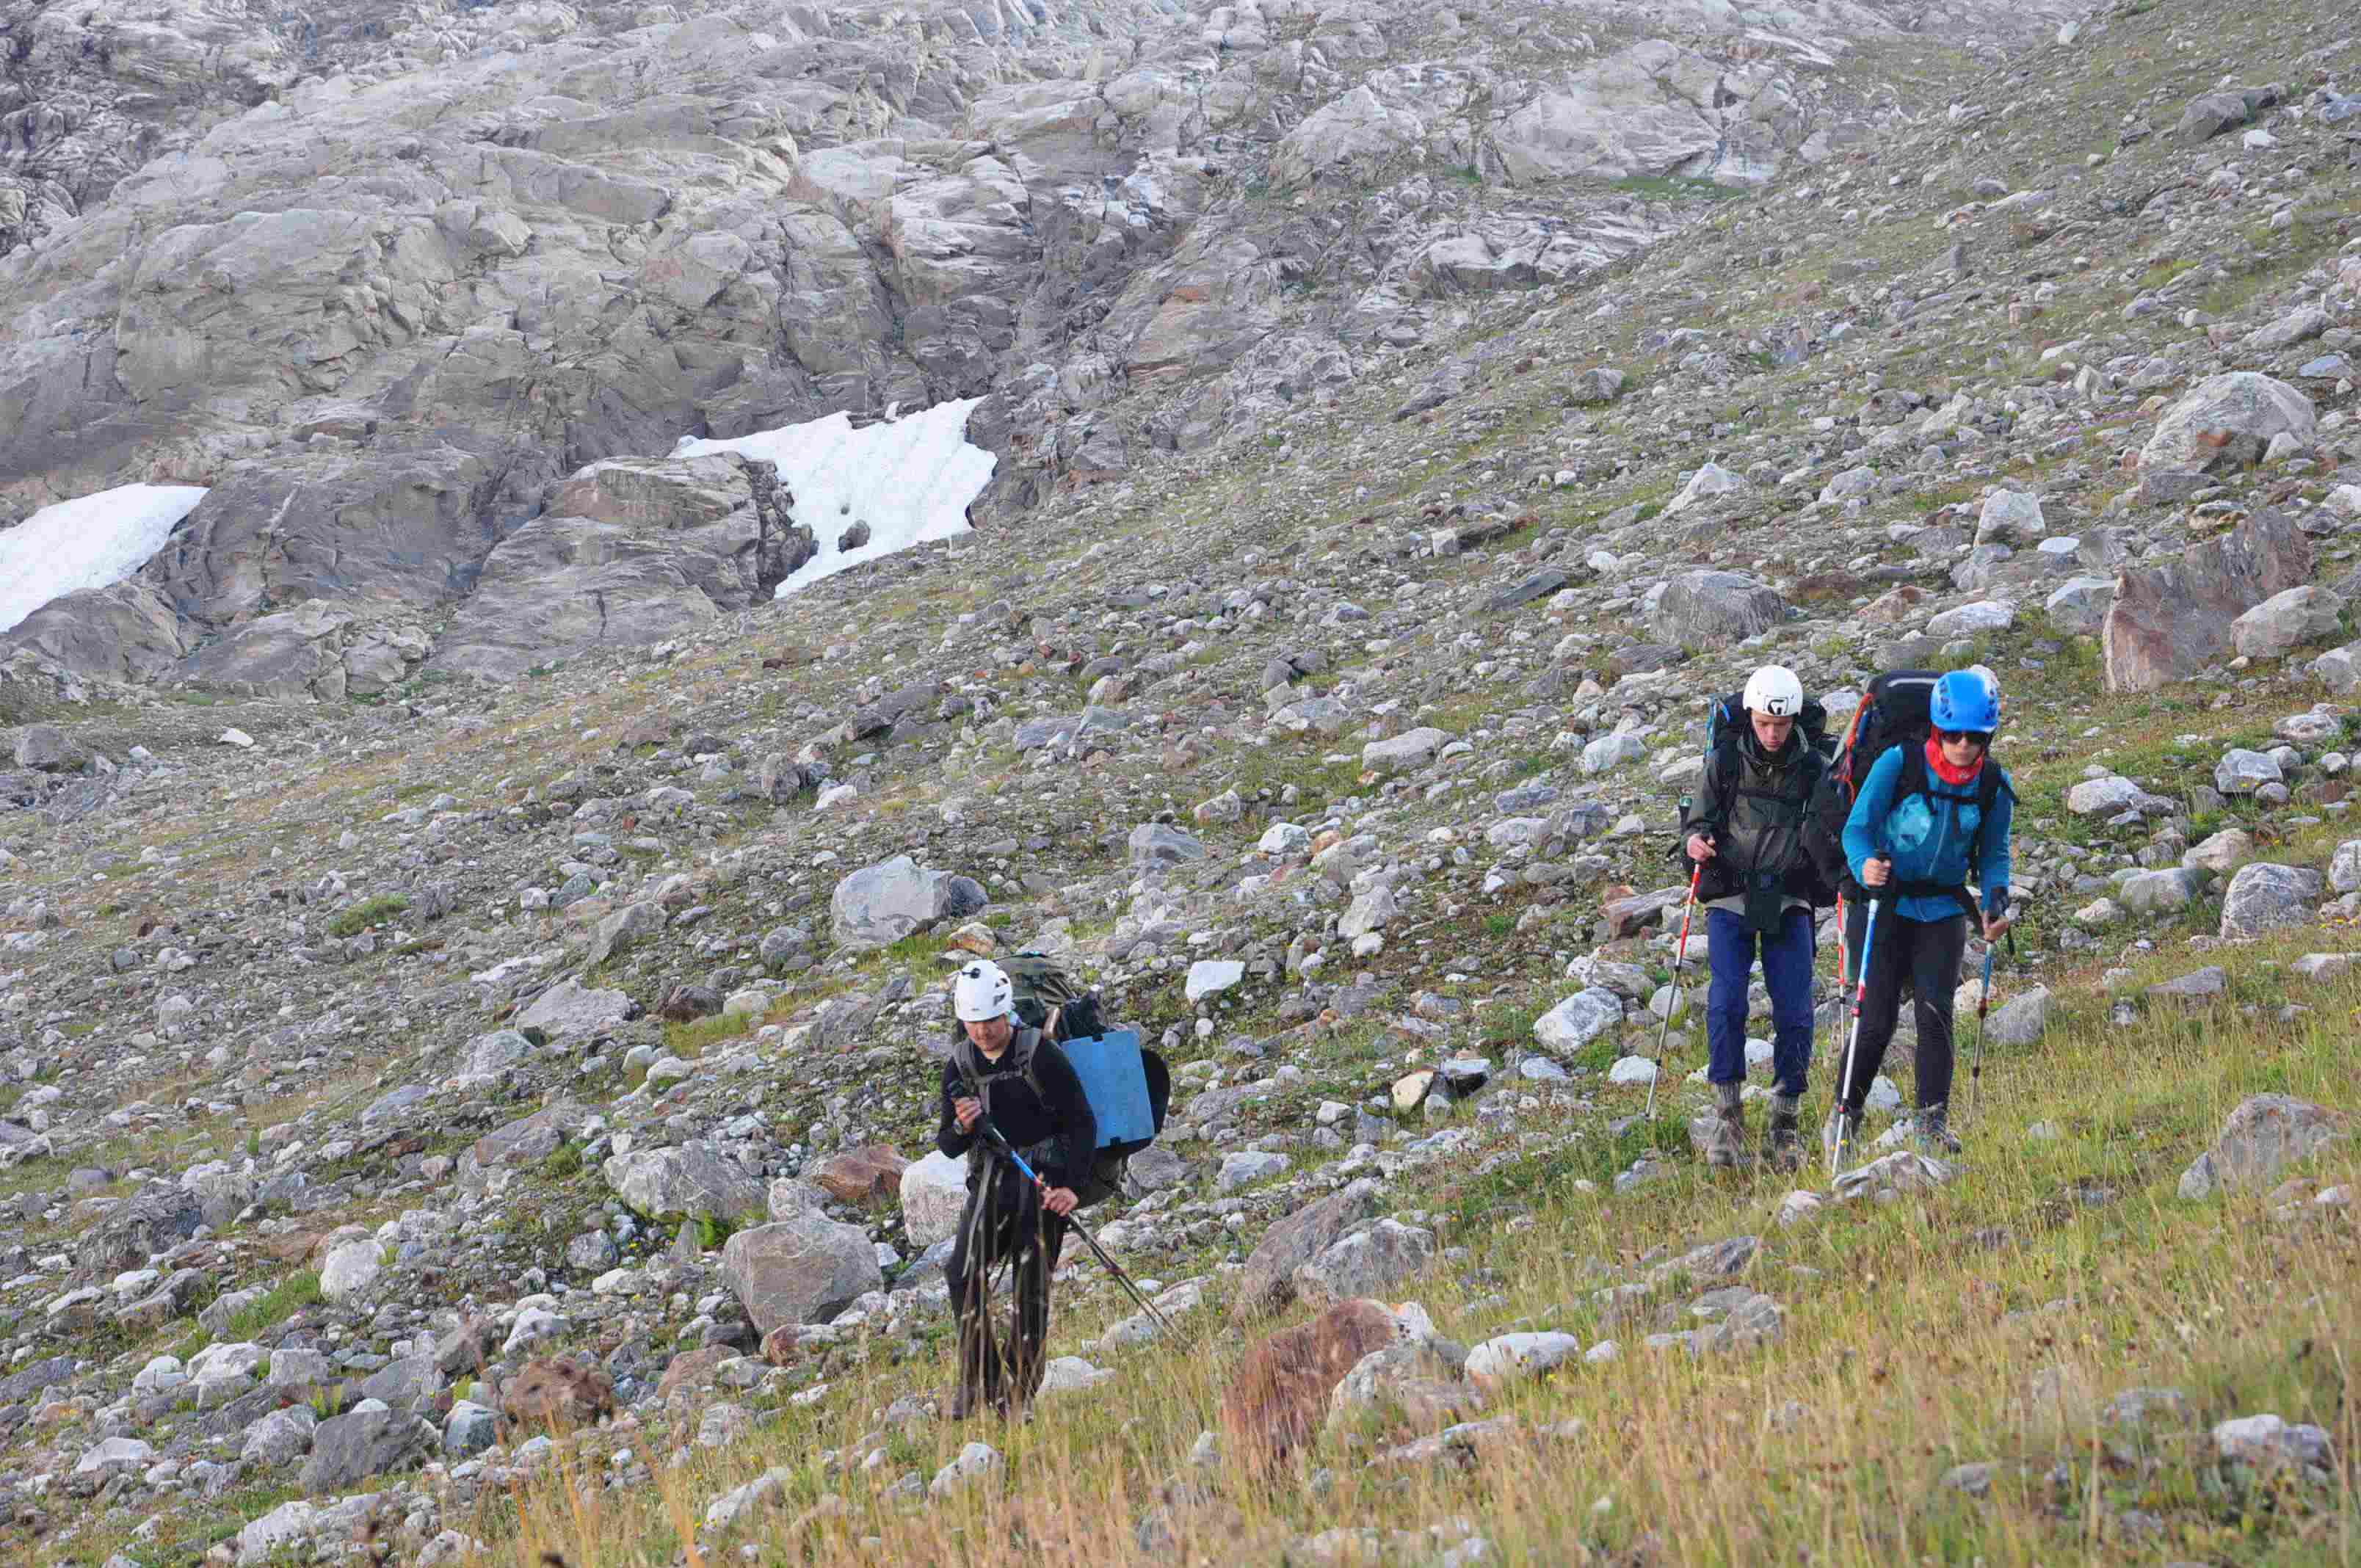
\includegraphics[width=\textwidth]{../pics/DSC_0430 2}			
\end{frame}

\begin{frame}
	\frametitle{Движение по курумнику. Фото Анучиной Светланы}
	\framesubtitle{День 10, 27 августа}
	\footnotesize Красная линия~--- наш трек
	\centering
	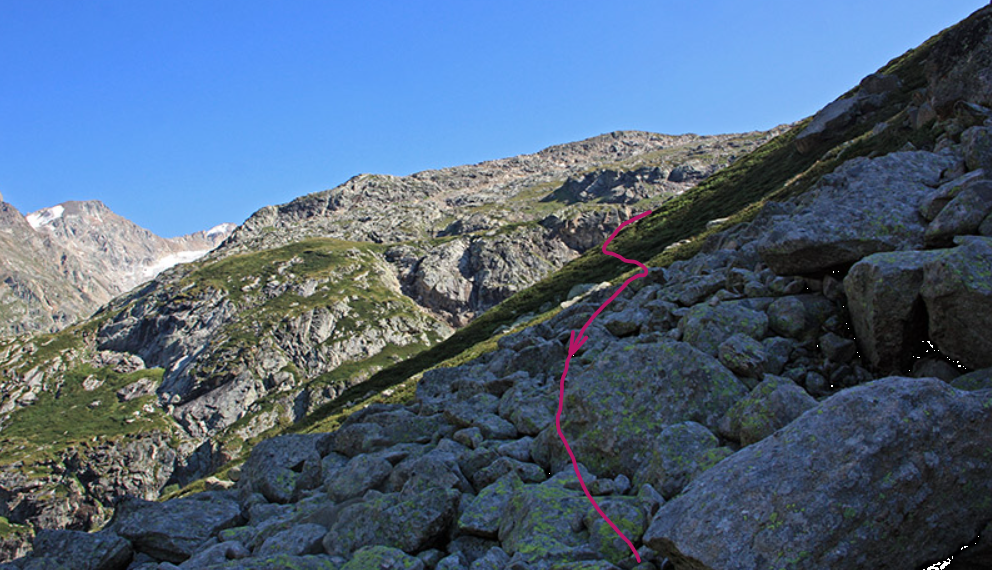
\includegraphics[width=\textwidth]{../pics/peremkurum.png}			
\end{frame}

